% =====================================================================
% Paper 9 - Direction-dependent band gaps in 2D anisotropic
% strain-gradient elastic media.
%
% STYLE-ADAPTED build.  Scientific content is byte-for-byte identical to
% the authoritative Paper9_FINAL_SOURCE_PACKAGE (OVERLEAF) manuscript;
% ONLY the publication/presentation layer follows the FEM_3 reference
% manuscript (elsarticle preprint layout, frontmatter, citation style,
% figure/table language, booktabs tables).  See ../REPORT/ for the full
% change record.  No equation, value, result, author, reference, or claim
% was altered.
% =====================================================================
\documentclass[preprint,12pt]{elsarticle}

%-------------------------------------------------
% Mathematics
%-------------------------------------------------
\usepackage{amsmath}
\usepackage{amssymb}
\usepackage{amsfonts}
\usepackage{bm}
\usepackage{mathtools}
\usepackage[a4paper,margin=1in]{geometry}

%-------------------------------------------------
% Figures and Tables
%-------------------------------------------------
\usepackage{graphicx}
\usepackage{booktabs}
\usepackage{multirow}
\usepackage{array}
\usepackage{tabularx}        % required by the Paper9 table fragments
\usepackage{subcaption}

%-------------------------------------------------
% Paper9 columns/lists required by the byte-identical sections:
%   \newcolumntype Y/L rely on \RaggedRight; sections use enumerate[label=...]
%-------------------------------------------------
\usepackage{ragged2e}
\newcolumntype{Y}{>{\RaggedRight\arraybackslash}X}
\newcolumntype{L}[1]{>{\RaggedRight\arraybackslash}p{#1}}
\usepackage{enumitem}

%-------------------------------------------------
% Units
%-------------------------------------------------
\usepackage{siunitx}

%-------------------------------------------------
% Colors
%-------------------------------------------------
\usepackage[table]{xcolor}

%-------------------------------------------------
% Hyperlinks (load near the end)
%-------------------------------------------------
\usepackage[hidelinks]{hyperref}

%-------------------------------------------------
% Barred and bold notations per project conventions (unchanged)
%-------------------------------------------------
\newcommand{\bmx}{\bm{x}}
\newcommand{\bmk}{\bm{k}}
\newcommand{\bmu}{\bm{u}}
\newcommand{\bmv}{\bm{v}}
\newcommand{\bmS}{\bm{S}}
\newcommand{\bmK}{\bm{K}}
\newcommand{\bmM}{\bm{M}}
\newcommand{\bmB}{\bm{B}}
\newcommand{\bmR}{\bm{R}}
\newcommand{\bmT}{\bm{T}}
\newcommand{\bmC}{\bm{C}}
\newcommand{\bmL}{\mathbf{L}}
\newcommand{\barw}{\bar{\omega}}
\newcommand{\bark}{\bar{k}}
\newcommand{\ellbar}{\bar{\ell}_{\mathrm{i}}}
\newcommand{\lbar}{\bar{l}}
\newcommand{\dif}{\mathrm{d}}
\newcommand{\iu}{\mathrm{i}}

\journal{International Journal of Mechanical Sciences}

\begin{document}

\begin{frontmatter}

%-------------------------------------------------
% Title
%-------------------------------------------------
\title{Direction-Dependent Band Gaps and Wave Steering in Two-Dimensional
Strain-Gradient Elastic Media with Anisotropic Ellipsoidal Microstructure:
A \texorpdfstring{Bloch--Floquet $C^1$}{Bloch--Floquet C1} Finite Element
Analysis}

%-------------------------------------------------
% Authors
%-------------------------------------------------
\author{Phase-1/P7 Collaborative Research Team\corref{cor1}}
\cortext[cor1]{Corresponding author.}
\address{Department of Mechanical Engineering / Metamaterials Laboratory}
\address{Haryana State Research Fund Project No.~14/66-2025 SPD/HSHEC/HSRF,
Session 2025--2026}

%-------------------------------------------------
% Abstract
%-------------------------------------------------
\begin{abstract}
Microstructured solids exhibit rich dispersive phenomena when acoustic
wavelengths approach characteristic internal length scales, where classical
local elasticity breaks down. While prior investigations of strain-gradient
metamaterials have largely been restricted to one-dimensional chains or
two-dimensional media with isotropic length scales, the role of
microstructural orientation as an independent design knob remains
unaddressed. In this work, we present a two-dimensional Bloch--Floquet
finite element framework for Mindlin Form-II strain-gradient elasticity
incorporating an anisotropic characteristic-length tensor derived from the
second moments of a rotated ellipsoidal averaging domain, alongside an
independent micro-inertia parameter $\ell_{\mathrm{i}}$. A
$C^1$-conforming Bogner--Fox--Schmit (BFS) 32-degree-of-freedom rectangular
element is formulated, wherein complex Bloch phase transformations are
consistently applied across nodal displacements as well as first-order and
mixed-second-order derivative degrees of freedom. The numerical
implementation is verified against an eight-test internal consistency suite
and mesh convergence across $4^2$ to $32^2$ elements, yielding an observed
empirical least-squares convergence rate of $p = 4.17$ (fitted over the
refinement levels admissible under a pre-declared measurement-resolution
rule; $95\%$ CI: $[3.15, 5.20]$; no theoretical order claimed) and a locked
operational numerical resolution floor of $\varepsilon_\Delta =
4.63 \times 10^{-11}$. In a homogeneous microstructured medium (Case H), we
demonstrate that microstructural anisotropy induces strong directional
frequency migration along $\Gamma$--$X$ while strictly preserving the
absence of complete omnidirectional band gaps ($\Delta_{\mathrm{complete}}
\le -0.3235$). The resulting $(\theta, \mathrm{AR})$ design map reveals an
orientation sensitivity metric $S_\theta$ that is largest at the most
elongated configuration ($2.34\,\mathrm{rad}^{-1}$ at $\mathrm{AR} = 10$),
accompanied by an acoustic wave-vector steering deviation of up to
$\delta_{\max} = 2.78^\circ$ at $\bar{k} = 0.5$ (invariant to within
$10^{-5}\,$deg over the full orientation grid $\theta \in [0^\circ,
90^\circ]$ at $\mathrm{AR}=10$, with the steering figure of merit
$M_s = \phi^*(90^\circ) - \phi^*(0^\circ)$ equal to $0^\circ$ at
$\mathrm{AR}=5$ and $10^\circ$ at $\mathrm{AR}=10$ on the locked $5^\circ$
sampling grid). Finally, asymptotic analysis and numerical evidence
demonstrate that micro-inertia is constitutively necessary to bound
high-wavenumber phase velocities to a finite horizon $v_{T,\infty} =
0.3162$, ensuring physical admissibility.
\end{abstract}

%-------------------------------------------------
% Keywords
%-------------------------------------------------
\begin{keyword}
Strain-gradient elasticity \sep Mindlin Form-II \sep Micro-inertia \sep
Bloch--Floquet analysis \sep $C^1$ Bogner--Fox--Schmit element \sep
Anisotropic length tensor \sep Directional band gaps \sep Wave steering
\end{keyword}

\end{frontmatter}

%-------------------------------------------------
% Highlights (retained from Paper9)
%-------------------------------------------------
\section*{Highlights}
\begin{itemize}
  \item Bloch--Floquet $C^1$ FE framework for 2D anisotropic strain-gradient elasticity.
  \item Rotated ellipsoidal neighborhood yields independent orientation $\theta$ and aspect ratio $\mathrm{AR}$.
  \item Consistent Bloch phase transformations applied to value and derivative DOFs.
  \item Micro-inertia is proved constitutively necessary to bound short-wave speeds.
  \item Directional stop bands and wave steering mapped over $(\theta, \mathrm{AR})$ design space.
\end{itemize}

%-------------------------------------------------
% Section inclusions
%-------------------------------------------------
\section{Introduction}
\label{sec:intro}

Periodic elastic media can be designed to control wave propagation through their dispersion. Early calculations established band structures for periodic composites; experiments and theory later showed that two-dimensional solids can support absolute acoustic gaps \cite{SigalasEconomou1992,kushwaha1993,vasseur2001}. Lattice analyses and topology-optimization studies have since used geometry to tailor pass bands, stop bands, and wave transmission \cite{MartinssonMovchan2003,SigmundJensen2003,Dalklint2022}. Recent methods target gaps at specified frequencies and use multiple materials to control gap formation, while scaling studies track how optimized gaps shift with structural size \cite{He2026,Nakayama2025,Quinteros2026}. Reviews cover phononic-crystal mechanisms, engineered band gaps, and applications \cite{Vasileiadis2021,Oudich2023,MaWangYuan2026}. A gap along selected directions does not guarantee a complete gap; the latter requires suppression throughout the Brillouin zone.

When a wavelength approaches the material's microstructural scale, a local Cauchy law may not capture size-dependent stiffness or dispersion. Higher-order theories add kinematic measures and their work-conjugate stresses. Their development draws on couple-stress and microstructure theories, second-gradient elasticity, and variational treatments of higher-order boundary work \cite{toupin1962,MindlinTiersten1962,mindlin1964,Mindlin1965,mindlineshel1968,Germain1973}. Later studies examined strain-gradient descriptions of nonuniform deformation and small-scale beam experiments \cite{Aifantis1999,YangChongLamTong2002,LamYangChongWangTong2003}. Reviews and lattice-based derivations describe other formulations of gradient elasticity \cite{askesaifantis2011,polyzosfotiadis2012}. We use the local Mindlin Form-II theory; nonlocal integral and micromorphic theories are related approaches, but they are distinct formulations.

A dynamic gradient model needs a kinetic-energy law as well as gradient stiffness. With classical inertia alone, the shear branch examined here has phase speed proportional to wavenumber at high wavenumbers. Independent gradient micro-inertia gives this branch a finite high-wavenumber limit. That result follows from the constitutive and kinetic-energy laws used here; other higher-order continua need not have the same limit. One-dimensional studies have examined dispersion in gradient-elastic beams and periodic media, including dipolar-gradient formulations \cite{papargyribeskou2009,liweizhou2016,HosseiniSladekSladekZhang2024}. A two-dimensional phononic crystal has also been analyzed with a relaxed micromorphic model that includes free and gradient micro-inertia \cite{MadeoColletMiniaciBillonOuisseNeff2018}. Together, these studies show that the continuum and inertia laws affect the interpretation of short-wavelength bands, although their constitutive models differ from the local Mindlin Form-II model used here.

Size-dependent phononic-crystal studies use a range of constitutive models. Transfer-matrix analyses show that imperfect interfaces can alter one-dimensional band gaps \cite{zhengwei2009}. Other one-dimensional work considers dipolar-gradient elasticity, gradient thermoelasticity, and flexoelectric strain-gradient coupling \cite{liweizhou2016,li2023anchorA,li2024anchorB,HosseiniSladekSladekZhang2024}. In two dimensions, researchers have applied nonlocal strain-gradient theory to nanoscale phononic crystals and studied mixed and defect modes in a phononic-crystal slab \cite{JinHuHu2022,JinHuHu2023}. Other model-specific comparisons include thermoelastic cylindrical crystals and functionally graded lattices \cite{hosseinizhang2021,mishra2026anchorC}. Anisotropy and orientation have also been studied in conventional phononic crystals: work on orthotropic fillers and anisotropic plates reports shifts in band locations and widths as material axes or inclusions rotate relative to the lattice \cite{zhanwei2010,YaoWuHouXin2011}. Recent studies examine direction-dependent gaps in anisotropic nanocrystal assemblies and the effects of anisotropic constituents in optimized phononic crystals \cite{Kim2023,Liu2024anisotropic}. For flexural plate waves, anisotropic equal-frequency contours can align group velocity with a lens interface over a broad frequency range \cite{Danawe2023}. Prior work has therefore established orientation-dependent band tuning. Here we examine how an oriented characteristic-length tensor affects dispersion and energy-flow direction in a local two-dimensional strain-gradient model with gradient micro-inertia.

The finite-element approximation must also accommodate the strain-gradient weak form. Because it contains second derivatives of displacement, the trial space must be $H^2$-conforming or use an equivalent mixed formulation. The bicubic Bogner--Fox--Schmit (BFS) rectangle provides $C^1$ continuity across elements on structured quadrilateral meshes \cite{bfs1965}. Earlier studies developed displacement-based, mixed, and implicit-gradient finite elements \cite{ShuKingFleck1999,AmanatidouAravas2002,ZervosPapanicolopulosVardoulakis2009,Beheshti2017}. Later work treats second-gradient boundary-value problems, higher-order Hermite mappings on regular and distorted domains, mixed elements with patch recovery or shared degrees of freedom, and mixed crack formulations \cite{AndreausDellIsolaGiorgioPlacidiLekszyckiRizzi2016,BacciocchiFantuzzi2023,BacciocchiFantuzzi2025,ChoiLeeSim2023,Papanicolopulos2024,ChirkovNazarenkoAltenbach2024}. For a conforming BFS Bloch element, the same phase transformation must be applied to displacement values and all derivative degrees of freedom, including the mixed derivative.

The studies cited above do not combine, in one two-dimensional Bloch--Floquet finite-element framework, a rotated ellipsoidal second-moment characteristic-length tensor, local Mindlin Form-II strain-gradient elasticity with independent gradient micro-inertia, and a conforming $C^1$ BFS discretization with phase transformations on all relevant degrees of freedom. This study addresses that combination and builds on established work on anisotropy, orientation effects, and size-dependent phononic crystals. It makes four contributions:
\begin{itemize}
  \item We formulate a Bloch--Floquet framework for two-dimensional anisotropic strain-gradient elasticity. The rotated ellipsoidal averaging domain defines the length tensor, with aspect ratio $\mathrm{AR}=l_1/l_2$ and orientation $\theta$ as separate design variables.
  \item Gradient micro-inertia is examined analytically and numerically. For the branch studied, $\ell_{\mathrm{i}}=0$ gives an unbounded high-wavenumber phase speed, whereas $\ell_{\mathrm{i}}>0$ yields the finite limit $v_{T,\infty}=\sqrt{\mu/\rho}\,l_{\mathrm{eff}}/(\sqrt{10}\,\ell_{\mathrm{i}})$ derived in \ref{app:asymptotics}.
  \item A conforming 32-degree-of-freedom BFS element is developed, with the same complex Bloch phase applied to displacement, first derivatives, and the mixed derivative.
  \item Across the $(\theta,\mathrm{AR})$ design space, we evaluate directional dispersion, gap measures, and group velocity. The energy-flux relation follows from local balance; the analysis also separates directional stop bands from complete gaps and measures steering amplitude and lobe orientation.
\end{itemize}

Section~\ref{sec:continuum} defines the anisotropic strain-gradient continuum and micro-inertia. Section~\ref{sec:bloch} sets out the Bloch--Floquet formulation, followed by the BFS discretization in Section~\ref{sec:fem}. Section~\ref{sec:verification} reports the analytical, numerical, and mesh checks. Section~\ref{sec:results} presents the homogeneous dispersion, directional gaps, design maps, steering, and the separate heterogeneous Case~C result; Section~\ref{sec:microinertia} examines the high-wavenumber response. Sections~\ref{sec:discussion} and~\ref{sec:conclusions} interpret the findings and state their limitations.

\section{Anisotropic Strain-Gradient Continuum with Micro-Inertia}
\label{sec:continuum}

\subsection{Ellipsoidal characteristic-length tensor}
In standard isotropic gradient elasticity, the microstructural influence is encapsulated by a single scalar length scale $l$. To represent an oriented microstructure, we define an ellipsoidal averaging neighborhood $\mathcal{E}$ in two dimensions with principal semi-axes $l_1$ and $l_2$:
\begin{equation}
\mathcal{E}_0 = \left\{ (x_1', x_2') \in \mathbb{R}^2 \;\middle|\; \frac{(x_1')^2}{l_1^2} + \frac{(x_2')^2}{l_2^2} \le 1 \right\},
\label{eq:ellipse_def}
\end{equation}
where $(x_1', x_2')$ denote local principal coordinates aligned with the microstructural symmetry axes. The second-moment characteristic-length tensor $\mathbf{L}_0$ associated with $\mathcal{E}_0$ is diagonal in the principal frame:
\begin{equation}
\mathbf{L}_0 = \begin{bmatrix} l_1^2 & 0 \\ 0 & l_2^2 \end{bmatrix}.
\label{eq:L0_mat}
\end{equation}
To preserve total averaging volume across microstructural distortions, we adopt a volume-equivalent (area-preserving) scaling rule referenced to an isotropic baseline length scale $l_{\mathrm{iso}}$:
\begin{equation}
l_1 = l_{\mathrm{iso}}\sqrt{\mathrm{AR}}, \quad l_2 = \frac{l_{\mathrm{iso}}}{\sqrt{\mathrm{AR}}}, \quad \det(\mathbf{L}_0) = l_1^2 l_2^2 = l_{\mathrm{iso}}^4 = \mathrm{const},
\label{eq:volume_equivalent}
\end{equation}
where $\mathrm{AR} = l_1/l_2 \ge 1$ denotes the microstructural aspect ratio.

\paragraph{Orientation and passive rotation.}
When the microstructural principal axes are rotated by an orientation angle $\theta$ relative to the global Cartesian coordinate frame $(x_1, x_2)$, the relationship between global coordinates $\bmx$ and local principal coordinates $\bmx'$ is given by the planar rotation matrix $\bmR(\theta)$:
\begin{equation}
\bmx' = \bmR(\theta)\bmx, \quad \bmR(\theta) = \begin{bmatrix} \cos\theta & \sin\theta \\ -\sin\theta & \cos\theta \end{bmatrix}.
\label{eq:R_matrix}
\end{equation}
Under passive coordinate transformation, the components of the characteristic-length tensor $\mathbf{L}(\theta)$ in the global coordinate frame are given by:
\begin{equation}
\mathbf{L}(\theta) = \bmR(\theta)^\mathsf{T} \mathbf{L}_0 \bmR(\theta) = \begin{bmatrix} \cos\theta & -\sin\theta \\ \sin\theta & \cos\theta \end{bmatrix} \begin{bmatrix} l_1^2 & 0 \\ 0 & l_2^2 \end{bmatrix} \begin{bmatrix} \cos\theta & \sin\theta \\ -\sin\theta & \cos\theta \end{bmatrix}.
\label{eq:L_rotation}
\end{equation}
Carrying out the matrix multiplication yields the explicit tensor components:
\begin{subequations}
\label{eq:L_components}
\begin{align}
L_{11}(\theta) &= l_1^2 \cos^2\theta + l_2^2 \sin^2\theta, \label{eq:L11} \\
L_{22}(\theta) &= l_1^2 \sin^2\theta + l_2^2 \cos^2\theta, \label{eq:L22} \\
L_{12}(\theta) &= L_{21}(\theta) = (l_2^2 - l_1^2)\cos\theta\sin\theta. \label{eq:L12}
\end{align}
\end{subequations}
Notice that for an elongated microstructure ($l_1 > l_2$), the off-diagonal coupling term $L_{12}(\theta)$ is strictly negative for $0 < \theta < 90^\circ$, reaching its extremum $(l_2^2 - l_1^2)/2$ at $\theta = 45^\circ$. Furthermore, because $\bmR(\theta)$ is an orthogonal transformation ($\bmR^\mathsf{T}\bmR = \mathbf{I}$), the eigenvalues of $\mathbf{L}(\theta)$ are strictly invariant under rotation:
\begin{equation}
\mathrm{spec}(\mathbf{L}(\theta)) \equiv \{l_1^2, l_2^2\} \quad \forall\,\theta \in [0, 2\pi).
\label{eq:eigenvalues_invariant}
\end{equation}
Consequently, positive definiteness $\bmv^\mathsf{T}\mathbf{L}(\theta)\bmv > 0$ for all non-zero vectors $\bmv \in \mathbb{R}^2$ is guaranteed independently of the orientation angle $\theta$.

\begin{figure}[htbp]
\centering
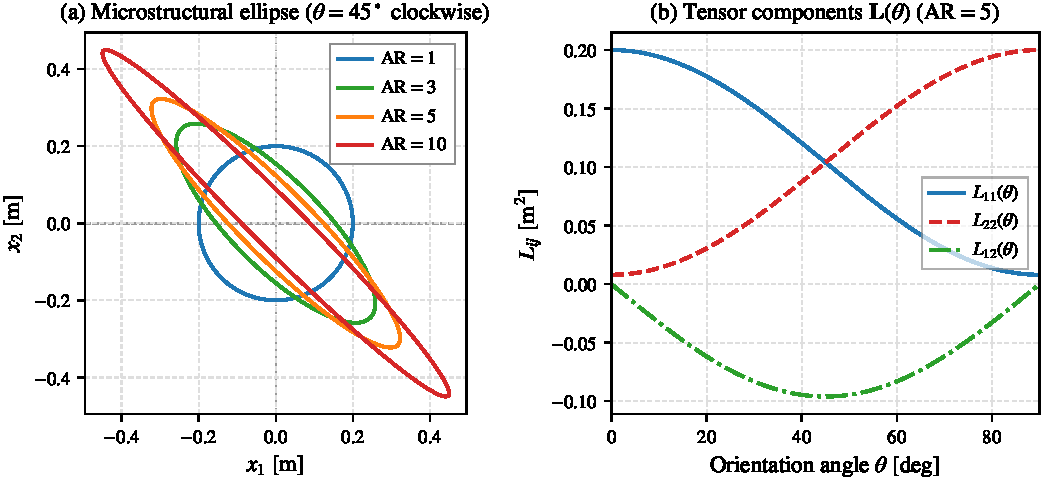
\includegraphics[width=\textwidth]{figures/fig01_ellipsoid_tensor.pdf}
\caption{(a) Volume-equivalent averaging ellipses at $\theta=45^\circ$ for $\mathrm{AR}=1,3,5,10$. (b) Length-tensor components versus orientation for $\mathrm{AR}=5$, including $L_{12}(45^\circ)=-0.096\,\mathrm{m}^2$ under the passive-rotation convention.}
\label{fig:ellipsoid_tensor}
\end{figure}

\subsection{Kinematics and constitutive response}
Assuming infinitesimal deformations under two-dimensional plane-strain conditions ($u_3 = 0, \partial(\cdot)/\partial x_3 = 0$), the classical displacement gradient and infinitesimal strain tensor $\bm\varepsilon$ are:
\begin{equation}
\varepsilon_{ij} = \frac{1}{2}(u_{i,j} + u_{j,i}), \quad i,j \in \{1, 2\}.
\label{eq:strain_def}
\end{equation}
In Mindlin's strain-gradient theory, the kinematic state includes the second displacement gradient or strain-gradient third-order tensor $\bm\eta$:
\begin{equation}
\eta_{ijk} = \varepsilon_{ij,k} = \frac{1}{2}(u_{i,jk} + u_{j,ik}), \quad \eta_{ijk} = \eta_{jik}.
\label{eq:strain_gradient_def}
\end{equation}
In 2D plane strain, the symmetric strain tensor $\bm\varepsilon$ contains 3 independent components ($\varepsilon_{11}, \varepsilon_{22}, 2\varepsilon_{12}$), while the strain-gradient tensor $\bm\eta$ possesses 6 independent components ($\eta_{111}, \eta_{112}, \eta_{221}, \eta_{222}, 2\eta_{121}, 2\eta_{122}$).

\paragraph{Mindlin Form-II constitutive law.}
We formulate the constitutive relations in Mindlin's Form II, wherein the strain energy density $W$ is decomposed into classical and higher-order strain-gradient contributions:
\begin{equation}
W = \frac{1}{2}\sigma_{ij}\varepsilon_{ij} + \frac{1}{2}\tau_{ijk}\eta_{ijk},
\label{eq:strain_energy_W}
\end{equation}
where $\bm\sigma$ is the Cauchy stress tensor and $\bm\tau$ is the third-order double-stress (or dipolar stress) tensor. For an isotropic base material parameterized by Lam\'e constants $\lambda$ and $\mu$, the Cauchy stress satisfies Hooke's law:
\begin{equation}
\sigma_{ij} = C_{ijkl}\varepsilon_{kl} = \lambda \delta_{ij}\varepsilon_{kk} + 2\mu \varepsilon_{ij}.
\label{eq:cauchy_stress}
\end{equation}
The double-stress tensor $\tau_{ijk}$ is conjugated to $\eta_{ijk}$ via an anisotropic gradient elasticity relation mediated by the characteristic-length tensor $\mathbf{L}$:
\begin{equation}
\tau_{ijk} = \frac{1}{10} L_{kl} C_{ijmn}\eta_{mnl} = \frac{1}{10} L_{kl}\left(\lambda \delta_{ij}\eta_{mml} + 2\mu \eta_{ijl}\right),
\label{eq:double_stress}
\end{equation}
where the prefactor $1/10$ arises from the second moment of the representative three-dimensional ellipsoidal averaging domain. Substituting Eq.~\eqref{eq:double_stress} into Eq.~\eqref{eq:strain_energy_W} demonstrates that $W$ is strictly non-negative and quadratic in both strains and strain gradients.

\paragraph{Gradient micro-inertia.}
To assess high-wavenumber regularization, the kinetic-energy density $T$ includes a gradient micro-inertia term:
\begin{equation}
T = \frac{1}{2}\rho \dot u_i \dot u_i + \frac{1}{2}\rho \ell_{\mathrm{i}}^2 \dot u_{i,j}\dot u_{i,j},
\label{eq:kinetic_energy_T}
\end{equation}
where $\rho$ is the macroscopic mass density and $\ell_{\mathrm{i}} > 0$ is the independent micro-inertia length parameter. Applying Hamilton's principle $\delta \int_{t_1}^{t_2} (T - W)\,\dif t = 0$ yields the strong-form equations of dynamic equilibrium in the bulk:
\begin{equation}
\sigma_{ij,j} - \tau_{ijk,jk} = \rho\left(\ddot u_i - \ell_{\mathrm{i}}^2 \ddot u_{i,jj}\right), \quad \text{in } \Omega.
\label{eq:strong_form}
\end{equation}
The Laplacian term $-\rho \ell_{\mathrm{i}}^2 \ddot u_{i,jj}$ on the right-hand side represents resistance to localized velocity gradients. For the shear branch examined here, Section~\ref{sec:steering} and Appendix~\ref{app:asymptotics} show that this term bounds the high-wavenumber phase speed.

\paragraph{Model reductions.}
The formulated anisotropic strain-gradient model contains four well-defined physical limits:
\begin{enumerate}[label=(\roman*)]
  \item \textbf{Classical Elasticity Limit ($l_m \to 0, \ell_{\mathrm{i}} \to 0$):} Double stresses vanish ($\tau_{ijk} \to 0$), micro-inertia vanishes, and the classical Navier equations of motion $\sigma_{ij,j} = \rho \ddot u_i$ are recovered with dispersionless acoustic speeds $c_T = \sqrt{\mu/\rho}$ and $c_L = \sqrt{(\lambda+2\mu)/\rho}$.
  \item \textbf{Isotropic Gradient Elasticity ($\mathrm{AR} = 1$):} Here $l_1 = l_2 = l_{\mathrm{iso}}$, so $L_{11} = L_{22} = l_{\mathrm{iso}}^2$ and $L_{12} = 0$ for all $\theta$, recovering isotropic Form-II gradient elasticity.
  \item \textbf{Gradient elasticity without micro-inertia ($\ell_{\mathrm{i}} = 0$):} Higher-order stiffness remains while dynamic regularization is removed; the transverse branch analyzed in Appendix~\ref{app:asymptotics} then has $v_p\propto k$ as $k\to\infty$.
  \item \textbf{Diagonal Rotation-Swap Symmetry ($\theta \to \theta + 90^\circ$ with $l_1 \leftrightarrow l_2$):} The components of $\mathbf{L}$ satisfy $L_{11}(\theta+90^\circ, l_1, l_2) = L_{22}(\theta, l_2, l_1)$ and $L_{12}(\theta+90^\circ, l_1, l_2) = -L_{12}(\theta, l_2, l_1)$, establishing rigorous rotational symmetry.
\end{enumerate}

\subsection{Boundary operators}
The variational formulation on boundary $\Gamma = \partial\Omega$ with unit outward normal $\bm n$ yields natural and essential boundary conditions:
\begin{equation}
p_i = \sigma_{ij}n_j - n_j n_k \tau_{ijk,k}, \quad R_i = n_j n_k \tau_{ijk},
\label{eq:traction_def}
\end{equation}
where $p_i$ is the effective surface traction and $R_i$ is the higher-order double traction. The corresponding work-conjugate kinematic variables are the displacement $u_i$ and the normal displacement derivative $\partial u_i/\partial n \equiv u_{i,j}n_j$.

\section{Bloch--Floquet formulation and observables}
\label{sec:bloch}

\subsection{Square lattice and Bloch conditions}
We generate the two-dimensional periodic medium by translating the square cell $\Omega_{\mathrm{cell}}=[0,L]\times[0,L]$ along
\begin{equation}
\bm{a}_1=\begin{bmatrix}L\\0\end{bmatrix},\qquad
\bm{a}_2=\begin{bmatrix}0\\L\end{bmatrix}.
\label{eq:lattice_vectors}
\end{equation}
The corresponding reciprocal vectors satisfy $\bm{a}_i\cdot\bm{b}_j=2\pi\delta_{ij}$:
\begin{equation}
\bm{b}_1=\frac{2\pi}{L}\begin{bmatrix}1\\0\end{bmatrix},\qquad
\bm{b}_2=\frac{2\pi}{L}\begin{bmatrix}0\\1\end{bmatrix}.
\label{eq:reciprocal_vectors}
\end{equation}
The first Brillouin zone is $\mathcal{B}=[-\pi/L,\pi/L]^2$. For the isotropic square lattice, $C_{4v}$ symmetry permits the path $\Gamma(0,0)$--$X(\pi/L,0)$--$M(\pi/L,\pi/L)$--$\Gamma$. Anisotropy reduces the symmetry to $C_{2v}$ for $\theta=0^\circ$ or $90^\circ$, and to $C_2$ at general orientation; full-zone measures are therefore evaluated over the corresponding Brillouin zone.

\begin{figure*}[!tbp]
\centering
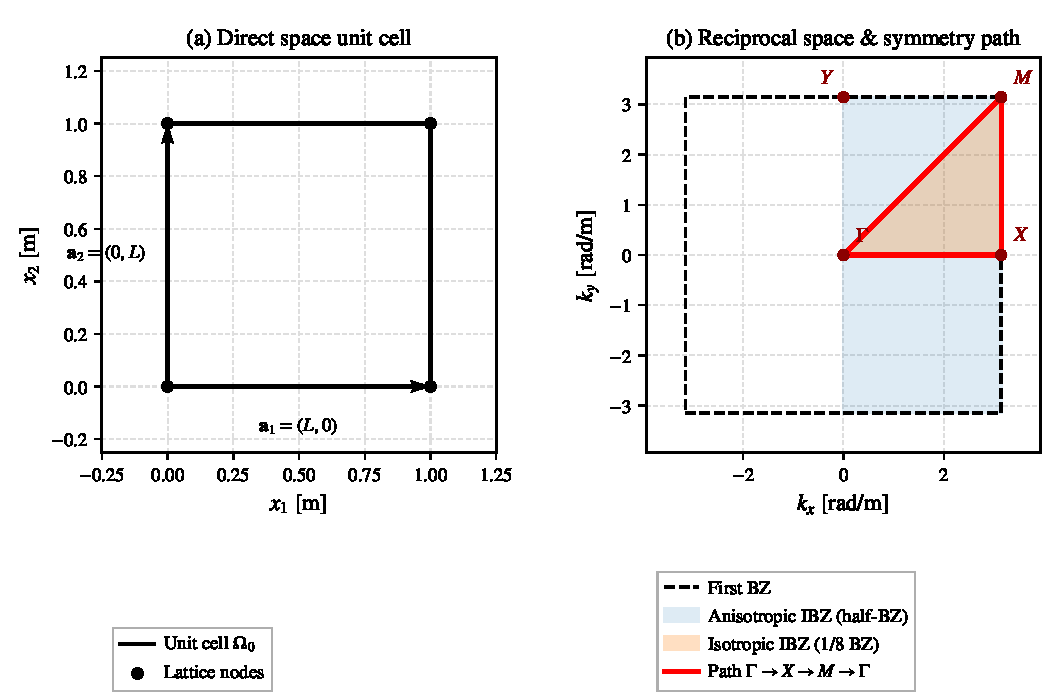
\includegraphics[width=\textwidth]{figures/fig02_lattice_ibz.pdf}
\caption{(a) Square periodic lattice. (b) First Brillouin zone and the high-symmetry contour $\Gamma$--$X$--$M$--$\Gamma$.}
\label{fig:lattice_ibz}
\end{figure*}

For a time-harmonic displacement $\bmu(\bmx,t)=\tilde{\bmu}(\bmx)e^{\iu(\bmk\cdot\bmx-\omega t)}$, Bloch periodicity gives
\begin{equation}
\bmu(\bmx+\bm{a}_\alpha)=\bmu(\bmx)e^{\iu\bmk\cdot\bm{a}_\alpha},\qquad \alpha\in\{1,2\}.
\label{eq:bloch_displacement}
\end{equation}
Because the approximation is $C^1$-conforming, differentiating the displacement relation gives:
\begin{equation}
\frac{\partial\bmu}{\partial x_\beta}(\bmx+\bm{a}_\alpha)=\frac{\partial\bmu}{\partial x_\beta}(\bmx)e^{\iu\bmk\cdot\bm{a}_\alpha},\qquad
\frac{\partial^2\bmu}{\partial x_1\partial x_2}(\bmx+\bm{a}_\alpha)=\frac{\partial^2\bmu}{\partial x_1\partial x_2}(\bmx)e^{\iu\bmk\cdot\bm{a}_\alpha}.
\label{eq:bloch_derivatives}
\end{equation}
Thus displacement, first derivatives, and cross derivatives all take the same Bloch phase; a different phase for derivative degrees of freedom would break $C^1$ continuity across cell boundaries.

\subsection{Nondimensionalization}
For Case~H, we scale length, frequency, and velocity with the cell length $L$, shear modulus $\mu$, and density $\rho$:
\begin{equation}
\bark=\frac{kL}{\pi},\qquad \barw=\frac{\omega}{\omega_0},\qquad
\omega_0=\sqrt{\frac{\mu}{\rho L^2}},\qquad
\bar{l}_m=\frac{l_m}{L},\qquad
\ellbar=\frac{\ell_{\mathrm{i}}}{L},\qquad
\bar{v}_p=\frac{\omega/k}{\sqrt{\mu/\rho}}.
\label{eq:nondim_defs}
\end{equation}
This gives $c_T=1$ and $c_L=\sqrt{(\lambda+2\mu)/\mu}=\sqrt{3}$ for $\lambda/\mu=1$ ($\nu=0.25$). Case~C uses the matrix shear speed and frequency scale specified in Table~\ref{tab:case_params}.

\subsection{Gap and steering measures}
At each wave vector, the eigenfrequencies are ordered as $\barw_1(\bmk)\le\barw_2(\bmk)\le\cdots$. We distinguish gaps evaluated on one path leg, the complete high-symmetry path, and the full Brillouin zone:
\begin{enumerate}[label=(\alph*)]
  \item \textbf{Leg gap:} for bands $n$ and $n+1$, $\Delta[\mathrm{leg}]=\min_{\bmk\in\mathrm{leg}}\barw_{n+1}(\bmk)-\max_{\bmk\in\mathrm{leg}}\barw_n(\bmk)$; $\Delta_{GX}$ denotes the $\Gamma$--$X$ leg.
  \item \textbf{Path gap:}
  \begin{equation}
  \Delta_{\mathrm{path}}=\min_{\bmk\in\mathrm{path}}\barw_{n+1}(\bmk)-\max_{\bmk\in\mathrm{path}}\barw_n(\bmk).
  \label{eq:delta_path}
  \end{equation}
  \item \textbf{Complete gap:}
  \begin{equation}
  \Delta_{\mathrm{complete}}=\min_{\bmk\in\mathcal{B}}\barw_{n+1}(\bmk)-\max_{\bmk\in\mathcal{B}}\barw_n(\bmk).
  \label{eq:delta_complete}
  \end{equation}
\end{enumerate}
Since the leg, path, and full zone are nested sets, $\Delta[\mathrm{leg}]\ge\Delta[\mathrm{path}]\ge\Delta[\mathrm{complete}]$:
\begin{equation}
\Delta[\mathrm{leg}]\ge\Delta[\mathrm{path}]\ge\Delta[\mathrm{complete}].
\label{eq:gap_hierarchy}
\end{equation}
A positive leg gap indicates directional filtering; a complete band gap requires $\Delta_{\mathrm{complete}}>0$.

The orientation sensitivity of a directional gap is measured by
\begin{equation}
S_\theta=\frac{\max_\theta\left|\frac{\partial\Delta}{\partial\theta}\right|}{\max_\theta\Delta}\quad[\mathrm{rad}^{-1}].
\label{eq:S_theta_def}
\end{equation}
The group velocity and its angular deviation from the wave vector are
\begin{equation}
\bmv_g=\nabla_{\bmk}\omega.
\label{eq:group_velocity}
\end{equation}
\begin{equation}
\delta=\angle\bmv_g-\angle\bmk.
\label{eq:steering_angle}
\end{equation}

\section{$C^1$ Finite Element Discretisation}
\label{sec:fem}

\subsection{Bogner--Fox--Schmit Bicubic Hermite Element}
In Mindlin Form-II gradient elasticity, the weak form of equilibrium requires square-integrable second derivatives of displacement, placing the variational space in the Sobolev space $H^2(\Omega)$. Consequently, standard $C^0$-continuous Lagrange elements are non-conforming and suffer from severe convergence pathologies. To guarantee conforming $C^1$ inter-element continuity across rectangular element boundaries, we adopt the Bogner--Fox--Schmit (BFS) bicubic element \cite{bfs1965}.

For a rectangular element of dimensions $2a \times 2b$, the displacement components $u_1(x, y)$ and $u_2(x, y)$ are interpolated independently as tensor products of one-dimensional cubic Hermite polynomials:
\begin{equation}
u_i(x, y) = \sum_{a=1}^4 \sum_{p=1}^4 N_{a,p}(x, y) d_{i, a, p}^e, \quad i \in \{1, 2\},
\label{eq:bfs_interpolation}
\end{equation}
where $a \in \{1, 2, 3, 4\}$ indexes the four element vertices, and $p \in \{1, 2, 3, 4\}$ denotes the four nodal degrees of freedom per displacement component:
\begin{equation}
\bm{d}_{i, a}^e = \begin{bmatrix} u_i & \frac{\partial u_i}{\partial x} & \frac{\partial u_i}{\partial y} & \frac{\partial^2 u_i}{\partial x \partial y} \end{bmatrix}^\mathsf{T}_{\text{at node } a}.
\label{eq:nodal_dof_vector}
\end{equation}
With 4 vertices and 2 displacement components, each BFS element contains $4 \times 2 \times 4 = 32$ degrees of freedom. Figure~\ref{fig:bfs_dof} illustrates the nodal DOF arrangement and the complex phase mapping on periodic boundaries. All band-structure and design-map results reported below are computed with a uniform mesh of $n \times n = 16 \times 16$ BFS elements per unit cell ($h = L/n = 0.0625$, hence $8 n^2 = 2048$ degrees of freedom per cell); the element order $n$ is listed in Table~\ref{tab:case_params}.

\begin{figure}[htbp]
\centering
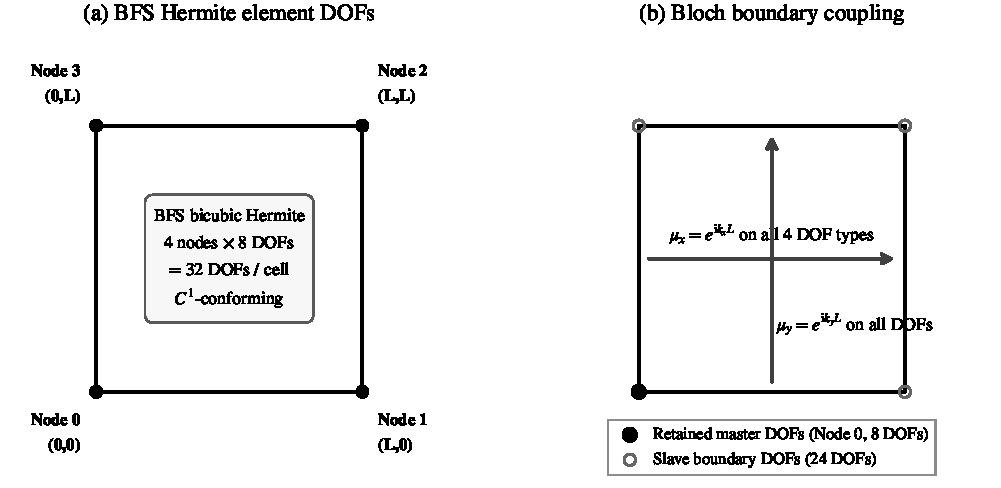
\includegraphics[width=\textwidth]{figures/fig03_bfs_dof_bloch.pdf}
\caption{(a) Degree-of-freedom structure of the 32-DOF $C^1$ Bogner--Fox--Schmit (BFS) bicubic element, showing 4 nodal DOFs $\{u, u_{,x}, u_{,y}, u_{,xy}\}$ per displacement component. (b) Master--slave Bloch periodic boundary coupling, illustrating identical phase transformation $e^{\iu \bmk \cdot \bm{a}_\alpha}$ applied across primary and derivative degrees of freedom.}
\label{fig:bfs_dof}
\end{figure}

\subsection{Element matrices}
The strain tensor $\bm\varepsilon$ and strain-gradient tensor $\bm\eta$ within element $e$ are related to the element nodal displacement vector $\bm{d}^e \in \mathbb{R}^{32}$ via kinematic strain-displacement matrices $\bmB^c$ and $\bmB^g_k$:
\begin{equation}
\bm\varepsilon = \bmB^c \bm{d}^e, \quad \bm\eta_k \equiv \frac{\partial \bm\varepsilon}{\partial x_k} = \bmB^g_k \bm{d}^e, \quad k \in \{1, 2\}.
\label{eq:strain_matrices}
\end{equation}
The total element stiffness matrix $\bmK^e$ separates cleanly into classical and gradient contributions:
\begin{equation}
\bmK^e = \bmK^c + \bmK^g(\theta, \mathrm{AR}),
\label{eq:Ke_total}
\end{equation}
where the classical stiffness matrix is:
\begin{equation}
\bmK^c = \int_{\Omega_e} (\bmB^c)^\mathsf{T} \bmC \bmB^c \,\dif\Omega,
\label{eq:Kc_int}
\end{equation}
and the anisotropic gradient stiffness matrix is:
\begin{equation}
\bmK^g(\theta, \mathrm{AR}) = \frac{1}{10} \sum_{k=1}^2 \sum_{l=1}^2 L_{kl}(\theta) \int_{\Omega_e} (\bmB^g_k)^\mathsf{T} \bmC \bmB^g_l \,\dif\Omega.
\label{eq:Kg_int}
\end{equation}
Because the shape functions are bicubic tensor-product polynomials, each homogeneous-element stiffness and mass integrand has degree at most six in each coordinate. A four-point Gauss--Legendre rule is exact through degree seven, so the $4 \times 4$ tensor rule is the smallest rule that integrates all such terms exactly. This avoids quadrature error for homogeneous elements; the unconstrained stiffness still has its expected rigid-body null modes. In elements cut by the inclusion, the discontinuous material field is instead integrated by sub-cell Gauss sampling with an $O(h)$ geometric approximation (Section~\ref{sec:caseC_pc}).

\paragraph{Mass and micro-inertia matrices.}
Similarly, the kinetic energy yields classical and micro-inertia mass contributions:
\begin{equation}
\bmM^e = \bmM_0 + \ell_{\mathrm{i}}^2 \bmM^g,
\label{eq:Me_total}
\end{equation}
with:
\begin{equation}
\bmM_0 = \rho \int_{\Omega_e} \bm{N}^\mathsf{T} \bm{N} \,\dif\Omega, \quad \bmM^g = \rho \sum_{k=1}^2 \int_{\Omega_e} \left(\frac{\partial \bm{N}}{\partial x_k}\right)^\mathsf{T} \left(\frac{\partial \bm{N}}{\partial x_k}\right) \,\dif\Omega.
\label{eq:Mg_int}
\end{equation}
Both $\bmM_0$ and $\bmM^g$ are symmetric and positive semi-definite; their sum $\bmM^e$ is strictly positive definite for any positive density $\rho > 0$.

\subsection{Bloch reduction and eigenproblem}
To apply the Bloch boundary conditions across the unit cell boundary $\partial\Omega_{\mathrm{cell}}$, the global degrees of freedom $\bm{d}$ are partitioned into interior ($I$), master boundaries ($M$), and slave boundaries ($S$):
\begin{equation}
\bm{d} = \begin{bmatrix} \bm{d}_I \\ \bm{d}_M \\ \bm{d}_S \end{bmatrix}.
\label{eq:d_partition}
\end{equation}
The slave degrees of freedom on the top and right boundaries are related to the corresponding master degrees of freedom on the bottom and left boundaries via the Bloch transformation:
\begin{equation}
\bm{d}_S = \bmT_{SM}(\bmk) \bm{d}_M,
\label{eq:slave_master_rel}
\end{equation}
where $\bmT_{SM}(\bmk)$ is a diagonal complex phase matrix formed by evaluating $e^{\iu k_x L}$, $e^{\iu k_y L}$, or $e^{\iu (k_x + k_y)L}$ for each periodic node pair. As derived in Section~\ref{sec:bloch}, identical phase factors apply to the displacement, first-order, and cross-derivative DOFs.

The continuous weak-form boundary work also cancels pairwise across opposite cell faces. The effective traction $p_i^{\mathrm{dyn}}$ defined in Section~\ref{sec:continuum} inherits the Bloch phase and reverses sign with the outward normal, while its test displacement carries the conjugate phase. The double traction $R_i=n_jn_k\tau_{ijk}$ inherits the Bloch phase but is unchanged by normal reversal; its work-conjugate normal derivative changes sign. Thus both face-work terms cancel. The associated line and corner terms pair under the same translations, including the product phase $e^{\iu(k_x+k_y)L}$ at the corner, so no independent free-boundary condition is imposed on a Bloch-paired face.

Defining the master-slave transformation matrix $\bmT(\bmk)$:
\begin{equation}
\bm{d} = \bmT(\bmk) \bar{\bm{d}}, \quad \bmT(\bmk) = \begin{bmatrix} \mathbf{I}_{II} & \mathbf{0} \\ \mathbf{0} & \mathbf{I}_{MM} \\ \mathbf{0} & \bmT_{SM}(\bmk) \end{bmatrix}, \quad \bar{\bm{d}} = \begin{bmatrix} \bm{d}_I \\ \bm{d}_M \end{bmatrix},
\label{eq:T_bloch}
\end{equation}
the reduced stiffness and mass matrices are obtained through Galerkin projection:
\begin{equation}
\bar{\bmK}(\bmk) = \bmT(\bmk)^\mathsf{H} \bmK \bmT(\bmk), \quad \bar{\bmM}(\bmk) = \bmT(\bmk)^\mathsf{H} \bmM \bmT(\bmk).
\label{eq:reduced_KM}
\end{equation}

\paragraph{Reduced Hermitian eigenproblem.}
The dispersion curves $\barw_n(\bmk)$ are determined by solving the reduced generalized eigenvalue problem:
\begin{equation}
\left[ \bar{\bmK}(\bmk) - \omega^2 \bar{\bmM}(\bmk) \right] \bar{\bm{d}} = \bm{0}.
\label{eq:eigenproblem}
\end{equation}
The diagonal phase subblock $\bmT_{SM}(\bmk)$ is unitary because each entry has unit modulus; the full map $\bmT(\bmk)$ is rectangular, has full column rank, and is not unitary. For positive elastic and inertial parameters, the full-cell matrices satisfy $\bmK\succeq 0$ and $\bmM\succ 0$. Their congruence projections therefore give Hermitian reduced operators:
\begin{equation}
\bar{\bmK}(\bmk)^\mathsf{H} = \bar{\bmK}(\bmk) \succeq 0, \quad \bar{\bmM}(\bmk)^\mathsf{H} = \bar{\bmM}(\bmk) \succ 0,
\label{eq:hermiticity}
\end{equation}
so the generalized eigenvalues $\omega_n^2$ are real and nonnegative. Furthermore, shifting $\bmk$ by a reciprocal lattice vector $\bm{G}$ leaves every Bloch phase unchanged and hence gives $\bar{\bmK}(\bmk + \bm{G}) = \bar{\bmK}(\bmk)$ and $\bar{\bmM}(\bmk + \bm{G}) = \bar{\bmM}(\bmk)$, ensuring exact periodicity across reciprocal space.

\paragraph{Branch tracking.}
Along high-symmetry path segments, band crossing occurs between modes of differing spatial symmetry. To maintain physical branch continuity and resolve mode identity, we employ the Modal Assurance Criterion (MAC) between modes at adjacent wave vectors $\bmk_1$ and $\bmk_2$. Let $\bm{d}_m(\bmk)=\bmT(\bmk)\bar{\bm{d}}_m(\bmk)$ be the corresponding full-cell eigenvector, and let $\bmM$ be the common, assembled full-cell mass matrix, including gradient micro-inertia. The cross-wavevector MAC is
\begin{equation}
\mathrm{MAC}_{mn}(\bmk_1,\bmk_2) = \frac{\left| \bm{d}_m(\bmk_1)^\mathsf{H} \bmM \bm{d}_n(\bmk_2) \right|^2}{\left( \bm{d}_m(\bmk_1)^\mathsf{H} \bmM \bm{d}_m(\bmk_1) \right) \left( \bm{d}_n(\bmk_2)^\mathsf{H} \bmM \bm{d}_n(\bmk_2) \right)}.
\label{eq:mac_def}
\end{equation}
Using lifted vectors gives both modes the same physical mass metric; the reduced mass matrix itself depends on $\bmk$ and is therefore not used as a common cross-wavevector metric. When the off-diagonal MAC indicates branch exchange, step-halving continuation is triggered. However, in accordance with standard phononic band-structure reporting, band gaps are formally evaluated using frequency-ordered eigenvalues $\barw_1(\bmk) \le \barw_2(\bmk) \le \dots \le \barw_N(\bmk)$, avoiding subjective mode-tracking ambiguities.

\section{Verification and numerical resolution}
\label{sec:verification}

We compare the implementation with analytical limits, independent transfer-matrix calculations, algebraic identities, and mesh-refinement results. For the published heterogeneous bilayers, we report only qualitative graphical agreement where source curves are available. Cases with ambiguous parameters or no numerical curves are not treated as external validation.

\subsection{Analytical limits and bilayer comparison}
In the isotropic homogeneous limit, the long-wavelength phase velocities recover the classical transverse and longitudinal speeds:
\begin{equation}
\lim_{k\to0}\frac{\omega_T(k)}{k}=\sqrt{\frac{\mu}{\rho}}=1.0,\qquad
\lim_{k\to0}\frac{\omega_L(k)}{k}=\sqrt{\frac{\lambda+2\mu}{\rho}}=\sqrt{3}\approx1.73205.
\label{eq:acoustic_limits}
\end{equation}
At $\bar{k}=0.001$, the computed acoustic speeds differ from these limits by $1.25\times10^{-8}$ (Table~\ref{tab:consistency_suite}). The pure-bending micro-beam reduction matches the published closed-form limits to within $10^{-15}$ \cite{papargyribeskou2009}; details appear in Supplementary Material~S2. The micro-inertia asymptote is checked separately in \ref{app:asymptotics} and Section~\ref{sec:microinertia}.

As a classical reference, we analyze a periodic AlN/BaTiO$_3$ bilayer with $a_A=a_B=0.01\,\mathrm{m}$ and $b=a_A+a_B=0.02\,\mathrm{m}$ using the Rytov relation \cite{li2024anchorB,zhengwei2009}:
\begin{equation}
\cos(Kb)=\cos(k_Aa_A)\cos(k_Ba_B)-\frac{1}{2}\left(\frac{Z_A}{Z_B}+\frac{Z_B}{Z_A}\right)\sin(k_Aa_A)\sin(k_Ba_B),
\label{eq:rytov}
\end{equation}
where $k_m=\omega\sqrt{\rho_m/c_{33,m}}$, $v_m=\sqrt{c_{33,m}/\rho_m}$, and $Z_m=\rho_m v_m$. The single-layer transfer-matrix identity and the identical-material bilayer reduction match their analytical limits to $6.47\times10^{-16}$ and $7.22\times10^{-16}$, respectively. The heterogeneous transfer-matrix trace reproduces the Rytov relation to $2.22\times10^{-16}$. The first three calculated stop-band intervals are $[0.4806,0.5209]$, $[0.9812,1.0215]$, and $[1.4993,1.5028]$ in normalized frequency. We compare the result with the published B1 plot visually because tabulated source data are unavailable; no percentage error is inferred from the curves.

We reproduce two gradient-elastic bilayer cases, but do not treat them as external validations. One published length-scale definition is dimensionally ambiguous. For the other, the plotted parameter set and normalization are unspecified, and the numerical curves are unavailable. Supplementary Material~S2 records these limitations and the status of each comparison. We also compare the dipolar layer matrix with the source's printed formulation; this checks the formulation but does not validate its band curves.

\subsection{Numerical consistency and mesh convergence}
The consistency checks assess operator Hermiticity, Brillouin-zone periodicity, isotropic rotational invariance, acoustic slopes, rotation--swap symmetry, matrix definiteness, the micro-inertia limit, and the energy-flux/group-velocity identity. Table~\ref{tab:consistency_suite} reports the values obtained for these comparisons. After the harmonic micro-inertia sign correction in Appendix~\ref{app:energy_flux}, the energy-flux residual cannot be independently recalculated because the raw harmonic fields are unavailable. We therefore retain this identity as an unresolved diagnostic rather than treating the reported residual as independent confirmation. Supplementary Material~S3 gives the check definitions and expanded diagnostics.

We assess mesh convergence for homogeneous Case~H on uniform $N\times N$ BFS grids, $N\in\{4,8,16,32\}$, at fixed $\bmk=(0.31\pi/L,0.22\pi/L)$. Figure~\ref{fig:mesh_convergence} shows the acoustic-frequency error relative to the closed-form value and the change between successive meshes. The fitted empirical rate is $p=4.17$ (95\% CI $[3.15,5.20]$) over the $4^2$, $8^2$, and $16^2$ levels. The reported $32^2$ result is resolution-limited and is excluded from the fit. This rate is empirical; it is not a theoretical-order claim. The operational mesh-change floor is $\varepsilon_\Delta=4.63\times10^{-11}$ and is distinct from eigensolver reproducibility. The smallest reported directional gap, $|\Delta_{GX}|=4.3\times10^{-3}$, exceeds the floor by approximately $9\times10^7$.

\begin{figure*}[!t]
\centering
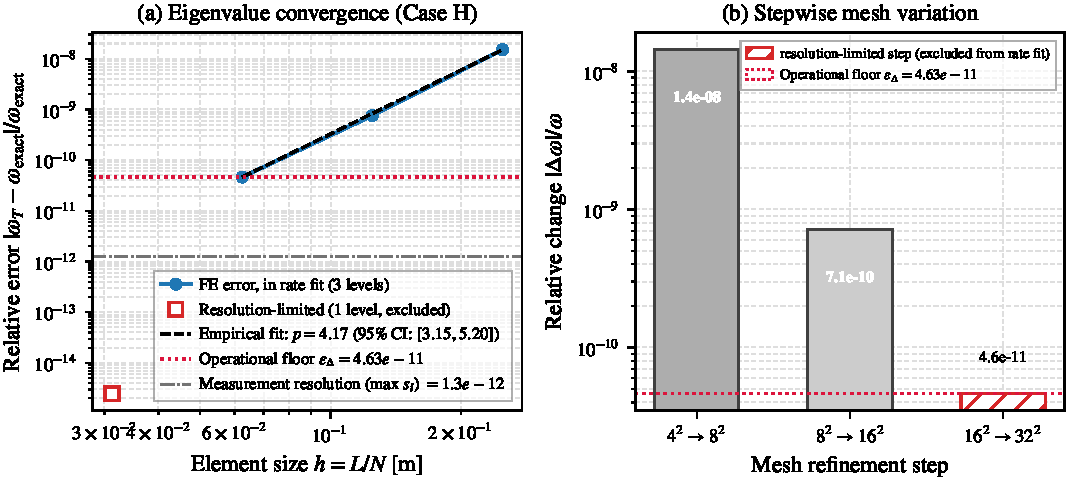
\includegraphics[width=\textwidth]{figures/fig05_mesh_convergence.pdf}
\caption{Case-H mesh study for the acoustic branch. (a) Relative frequency error versus element size; the $32^2$ result is shown as resolution-limited and is not included in the empirical fit. (b) Successive-mesh change and the operational mesh-change floor $\varepsilon_\Delta$.}
\label{fig:mesh_convergence}
\end{figure*}

\begin{table*}[!t]
\centering
\caption{Numerical consistency checks for the Bloch finite-element implementation.}
\label{tab:consistency_suite}
\begin{tabularx}{\textwidth}{@{}l Y c c c@{}}
\toprule
Check & Quantity assessed & Maximum discrepancy & Criterion & Result \\
\midrule
Hermiticity & Reduced stiffness and mass operators & $2.01\times10^{-16}$; $5.63\times10^{-17}$ & $<10^{-12}$ & Within criterion \\
Brillouin-zone periodicity & Spectrum under reciprocal-lattice shifts & $9.66\times10^{-16}$ & $<10^{-10}$ & Within criterion \\
Isotropic rotation & Frequencies at $\mathrm{AR}=1$ & $9.63\times10^{-16}$ & $<10^{-10}$ & Within criterion \\
Acoustic limit & Long-wave transverse and longitudinal slopes & $1.25\times10^{-8}$ & $<10^{-6}$ & Within criterion \\
Rotation--swap symmetry & Spectrum under $\theta\mapsto\theta+90^\circ$ and axis swap & $6.44\times10^{-16}$ & $<10^{-10}$ & Within criterion \\
Definiteness & Two rigid modes at $\Gamma$; positive interior spectrum & As expected & Admissible & As expected \\
Micro-inertia limit & Phase speed at $\bar{k}=200$ versus asymptotic value & $2.85\times10^{-4}$ & $<10^{-3}$ & Within criterion \\
Energy-flux identity & Group velocity versus cycle-averaged flux & $6.91\times10^{-10}$ & $<10^{-6}$ & Unresolved \\
\bottomrule
\end{tabularx}

\end{table*}

Selected Case-H and Case-C inputs appear with the Results. Supplementary Material~S1--S4 contains the full parameter summary, external-comparison details, and extended convergence diagnostics.

\section{Dispersion and directional filtering}
\label{sec:results}

The results separate two mechanisms: Case~H isolates the effect of an oriented characteristic-length tensor in a homogeneous medium, whereas Case~C adds periodic material contrast. The first controls direction-dependent dispersion and steering; the second can open a complete gap, although its reported width is mesh-sensitive. Selected inputs are summarized in Table~\ref{tab:case_params}; the extended parameter set is given in Supplementary Material~S1.

\begin{table}[htbp]
\centering
\caption{Selected material and numerical inputs for Cases H and C and the steering analysis.}
\label{tab:case_params}
\begin{tabularx}{\textwidth}{@{}l p{3.0cm} Y@{}}
\toprule
Case & Quantity & Value \\
\midrule
H & Cell and matrix & $L=1.0\,\mathrm{m}$; $\lambda=\mu=1.0\,\mathrm{Pa}$; $\rho=1.0\,\mathrm{kg/m^3}$ \\
H & Lengths and mesh & $l_{\mathrm{iso}}=0.20\,\mathrm{m}$; $\ell_{\mathrm{i}}=0.20\,\mathrm{m}$; $16\times16$ BFS elements per cell \\
C & Epoxy matrix & $\rho_m=1142\,\mathrm{kg/m^3}$; $\mu_m=1.48\,\mathrm{GPa}$; $\lambda_m=4.57\,\mathrm{GPa}$ \\
C & YBCO inclusion & $\rho_i=6333\,\mathrm{kg/m^3}$; $\mu_i=37.0\,\mathrm{GPa}$; $\lambda_i=95.0\,\mathrm{GPa}$ \\
C & Geometry and length scales & $L=1.0\,\mathrm{m}$; $r_0/L=0.30$; $\ell_m/L=0.10$; $\ell_i/L=0.20$ \\
C & Frequency scale and reported resolution & $c_{t,m}=1138.4\,\mathrm{m/s}$; $\omega_{0,C}=\pi c_{t,m}/L=3576.4\,\mathrm{rad/s}$; $4\times4$ mesh and $21\times21$ zone grid \\
Steering & Acoustic-branch sweep & $\bar{k}=0.5$; $\mathrm{AR}\in\{5,10\}$; $\theta=0^\circ,15^\circ,\ldots,90^\circ$ \\
\bottomrule
\end{tabularx}

\end{table}

\subsection{Anisotropy reshapes the homogeneous spectrum}
Figure~\ref{fig:caseH_dispersion} compares the isotropic reference with two orientations of the anisotropic length tensor. Both acoustic branches emerge from zero frequency at $\Gamma$, while changes in aspect ratio and orientation shift the branches and lift symmetry-related degeneracies at the zone edge. For $\mathrm{AR}=10$ and $\theta=45^\circ$, a narrow stop band opens along $\Gamma$--$X$, with $\Delta_{GX}=0.0043$. It is directional rather than complete: modes on other propagation directions overlap this interval, and the full-zone complete-gap measure remains $\Delta_{\mathrm{complete}}\le -0.3235$.

\begin{figure}[htbp]
\centering
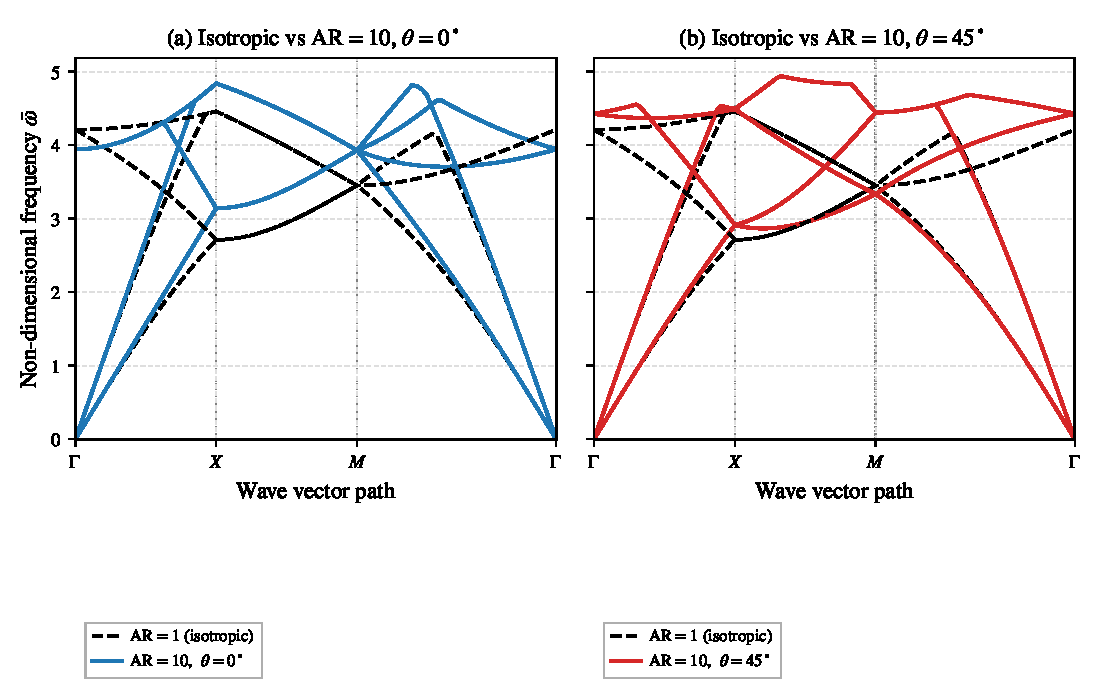
\includegraphics[width=\textwidth]{figures/fig06_caseH_dispersion.pdf}
\caption{Case-H Bloch bands along $\Gamma$--$X$--$M$--$\Gamma$. (a) Isotropic reference ($\mathrm{AR}=1$) and aligned anisotropy ($\mathrm{AR}=10$, $\theta=0^\circ$). (b) Isotropic reference and diagonal anisotropy ($\mathrm{AR}=10$, $\theta=45^\circ$), which opens a $\Gamma$--$X$ stop band but no complete gap.}
\label{fig:caseH_dispersion}
\end{figure}

The orientation sweep in Figure~\ref{fig:theta_sweep} shows how rotation redistributes the zone-edge frequencies. At $\mathrm{AR}=5$, as $\theta$ changes from $0^\circ$ to $90^\circ$, the transverse and longitudinal frequencies at $X$ decrease from $2.915$ to $2.672$ and from $5.050$ to $4.628$, respectively, as the projected length scale changes from the major to the minor axis. The $M$-point frequencies exhibit reflection symmetry about $45^\circ$, consistent with the square-cell symmetry.

\begin{figure}[htbp]
\centering
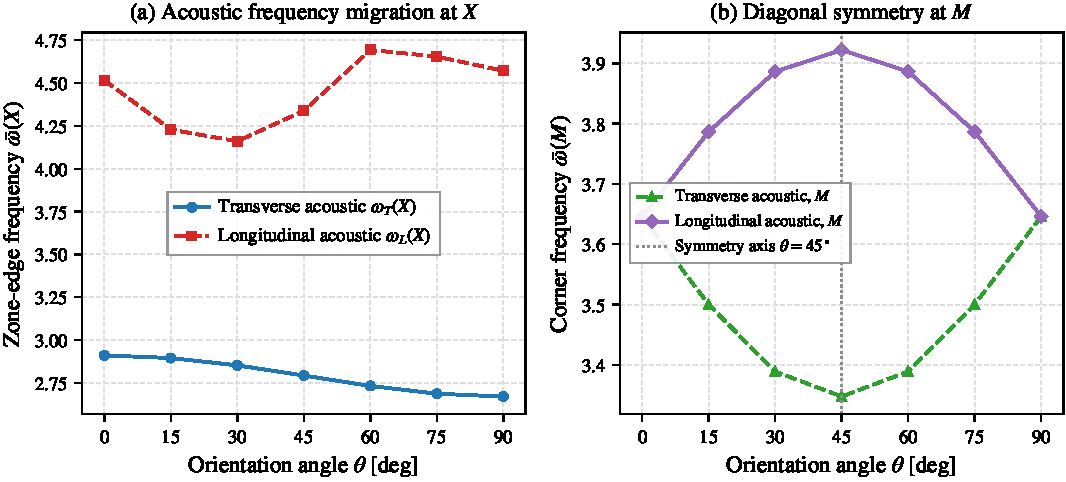
\includegraphics[width=\textwidth]{figures/fig08_theta_sweep.pdf}
\caption{Orientation dependence of the first four Case-H eigenfrequencies at (a) $X$ and (b) $M$ for $\mathrm{AR}=5$. The $M$-point response is symmetric about $\theta=45^\circ$.}
\label{fig:theta_sweep}
\end{figure}

Figure~\ref{fig:ar_sweep} isolates the effect of elongation at $\theta=45^\circ$. The isotropic case already has an orientation-independent directional width $\Delta_{GX}=0.041$; increasing $\mathrm{AR}$ changes the relative branch positions, but the directional gap is not monotone in aspect ratio.

\begin{figure}[htbp]
\centering
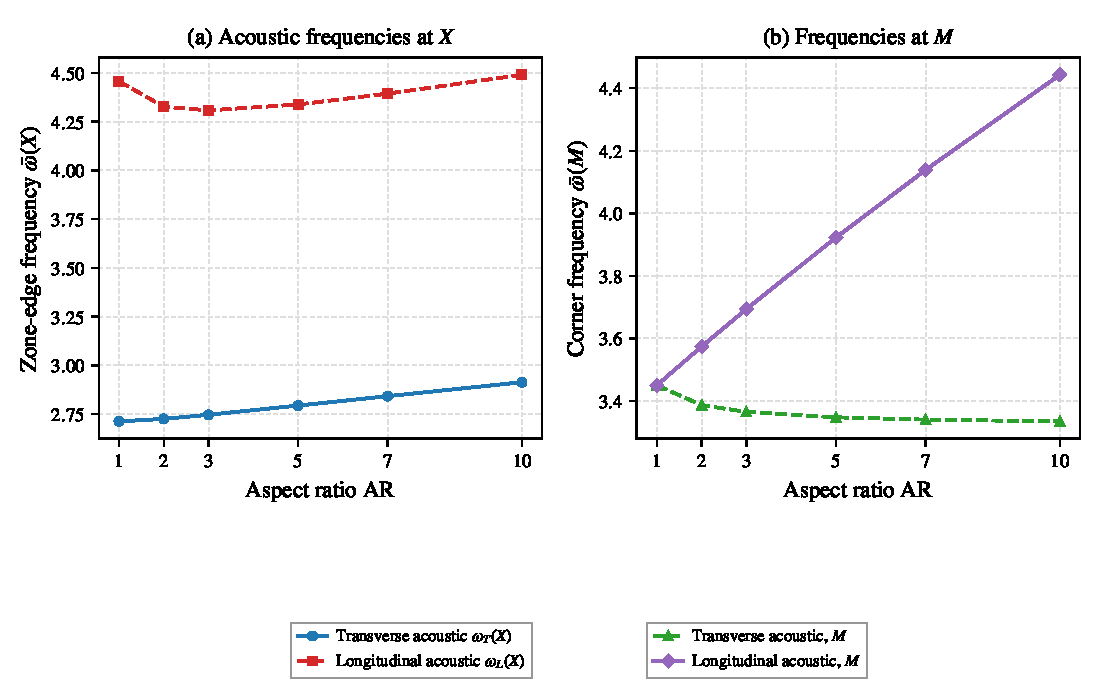
\includegraphics[width=\textwidth]{figures/fig09_ar_sweep.pdf}
\caption{Case-H branch frequencies at $X$ and $M$ as the aspect ratio varies from $1$ to $10$ at fixed $\theta=45^\circ$, using volume-equivalent length scaling.}
\label{fig:ar_sweep}
\end{figure}

The combined $(\theta,\mathrm{AR})$ sample in Figure~\ref{fig:design_map} identifies a maximum $\Delta_{GX}=0.0677$ at $(0^\circ,7)$ among 42 evaluated configurations; the response is non-monotone in aspect ratio. The plotted surface interpolates these evaluated points and is not a continuous optimization. The polar view in Figure~\ref{fig:polar_map} recasts the same sampled values by the sign of $\Delta_{GX}$; its regime boundary is descriptive of the sampled response.

\begin{figure}[htbp]
\centering
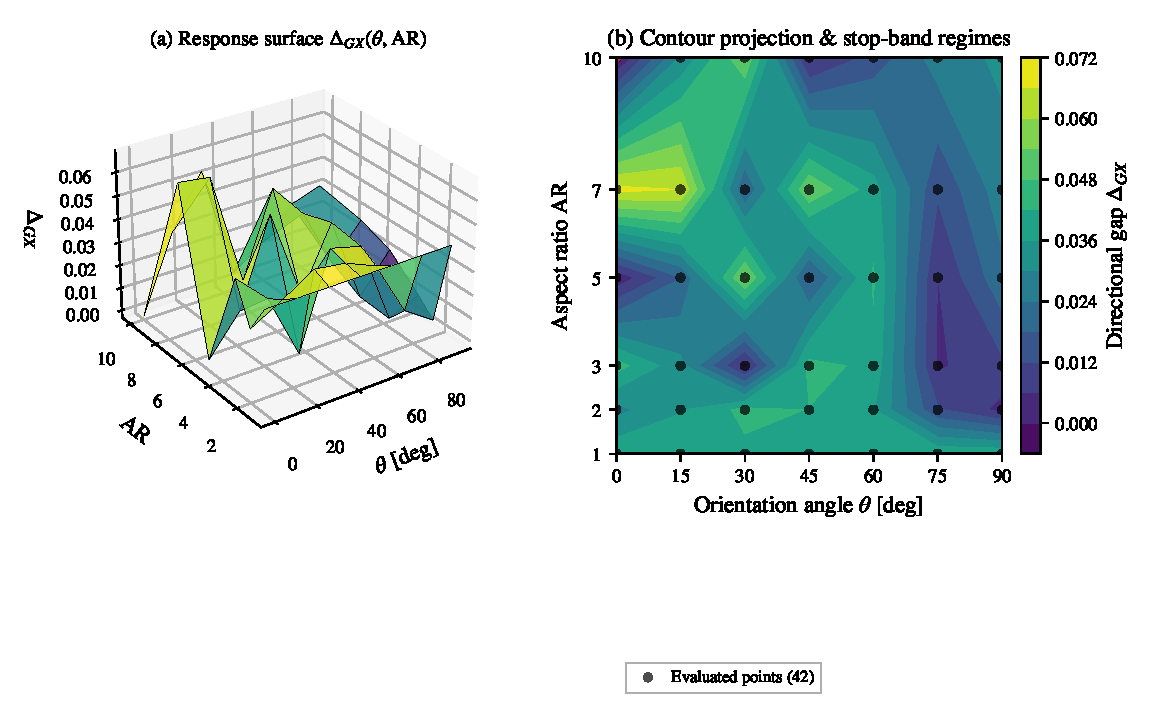
\includegraphics[width=\textwidth]{figures/fig10_design_map_3d.pdf}
\caption{Sampled Case-H design response $\Delta_{GX}(\theta,\mathrm{AR})$ for 42 configurations. The largest sampled value is $0.0677$ at $\theta=0^\circ$, $\mathrm{AR}=7$; at $\theta=45^\circ$, $\mathrm{AR}=10$, $\Delta_{GX}=0.0043$.}
\label{fig:design_map}
\end{figure}

\begin{figure}[htbp]
\centering
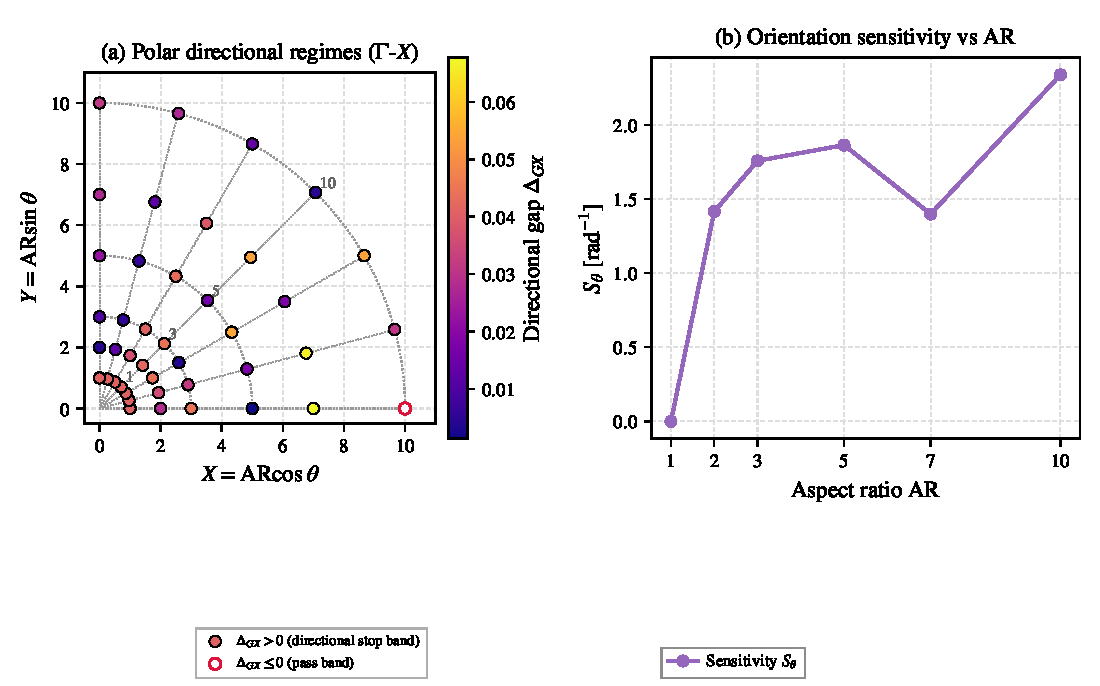
\includegraphics[width=\textwidth]{figures/fig11_polar_map_regimes.pdf}
\caption{Polar-coordinate view of the sampled Case-H designs, classified by $\Delta_{GX}\le0$ (pass band) and $\Delta_{GX}>0$ (directional stop band). The displayed boundary is a visual summary of sampled points.}
\label{fig:polar_map}
\end{figure}

Table~\ref{tab:gap_summary} summarizes representative directional and complete-gap measures. The complete-gap values remain negative for every listed homogeneous configuration, while the orientation sensitivity $S_\theta$ is largest at $\mathrm{AR}=10$ ($2.34\,\mathrm{rad}^{-1}$). The normalized widths and mesh-to-mesh variations are reported in Supplementary Material~S3.

\begin{table}[htbp]
\centering
\caption{Directional and complete-gap measures for representative Case-H configurations; values are reported at the precision retained between the $8\times8$ and $16\times16$ meshes.}
\label{tab:gap_summary}
\begin{tabularx}{\textwidth}{@{}c c r r r@{}}
\toprule
$\mathrm{AR}$ & $\theta$ & $\Delta_{GX}$ & $\Delta_{\mathrm{path}}$ & $\Delta_{\mathrm{complete}}$ \\
\midrule
$1$ & $0^\circ$  & $+0.041$ & $-0.32$ & $-0.32$ \\
$1$ & $45^\circ$ & $+0.041$ & $-0.32$ & $-0.32$ \\
$1$ & $90^\circ$ & $+0.041$ & $-0.32$ & $-0.32$ \\
$3$ & $0^\circ$  & $+0.045$ & $-0.10$ & $-0.46$ \\
$3$ & $45^\circ$ & $+0.044$ & $-0.45$ & $-0.48$ \\
$3$ & $90^\circ$ & $+0.011$ & $-0.33$ & $-0.46$ \\
$5$ & $0^\circ$  & $+0.001$ & $-0.01$ & $-0.58$ \\
$5$ & $45^\circ$ & $+0.016$ & $-0.48$ & $-0.58$ \\
$5$ & $90^\circ$ & $+0.022$ & $-0.37$ & $-0.58$ \\
$10$ & $0^\circ$  & $-0.002$ & $-0.24$ & $-0.85$ \\
$10$ & $45^\circ$ & $+0.004$ & $-0.29$ & $-0.56$ \\
$10$ & $90^\circ$ & $+0.031$ & $-0.65$ & $-0.85$ \\
\midrule
\multicolumn{5}{@{}l@{}}{$S_\theta$ [rad$^{-1}$]: AR $=1$: $0.00$; $2$: $1.42$; $3$: $1.76$; $5$: $1.86$; $7$: $1.40$; $10$: $2.34$.} \\
\bottomrule
\end{tabularx}

\end{table}

\subsection{Periodic material contrast opens a complete gap}
\label{sec:caseC_pc}
Unlike homogeneous Case~H, Case~C combines gradient elasticity with a periodic epoxy--YBCO impedance contrast ($\chi_\mu=25.0$, $\chi_\rho=5.546$; Table~\ref{tab:case_params}). The cell period is denoted $L$ here and $a$ in Figure~\ref{fig:caseC_dispersion}; $r_0/L=r_0/a=0.30$ gives a filling fraction of $28.27\%$. Figure~\ref{fig:caseC_dispersion} shows a complete gap between Bands~3 and~4 over $\bar{\omega}\in[4.5698,7.1430]$, giving $\Delta_{\mathrm{complete}}=2.5732$ or $43.94\%$ on the $4\times4$ mesh and $21\times21$ Brillouin-zone grid. The circular interface is integrated by sub-cell Gauss sampling on the Cartesian mesh. Brillouin-zone refinement changes the quoted width by less than $4\times10^{-4}$, but finite-element refinement has a much larger effect.

\begin{figure}[htbp]
\centering
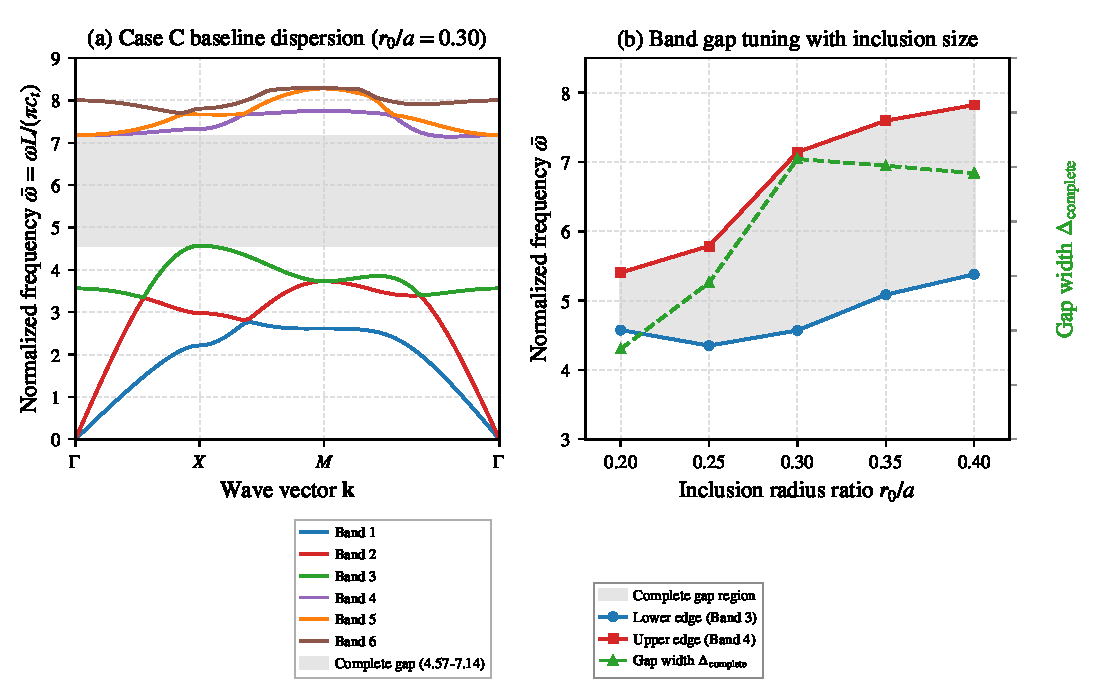
\includegraphics[width=\textwidth]{figures/fig07_caseC_dispersion.pdf}
\caption{Case-C complete-gap formation and radius dependence. (a) Bands along $\Gamma$--$X$--$M$--$\Gamma$ for $r_0/L=0.30$, with the $4\times4$-mesh gap between Bands~3 and~4. (b) Complete-gap width versus $r_0/a$ at the same mesh; the $r_0/a=0.30$ result is not mesh-converged.}
\label{fig:caseC_dispersion}
\end{figure}

The complete gap decreases monotonically from $2.5732$ at $4\times4$ to $2.2504$, $2.0722$, $1.9736$, and $1.9179$ at $8\times8$, $16\times16$, $32\times32$, and $64\times64$, respectively. It remains open at each computed resolution but is not mesh-converged; $2.5732$ is therefore a coarse-mesh result, not a converged continuum value. At the $4\times4$ mesh, increasing $r_0/L$ from $0.20$ to $0.30$ widens the gap from $0.8288$ ($16.61\%$) to $2.5732$ ($43.94\%$), after which it narrows to $2.4426$ ($37.00\%$) at $r_0/L=0.40$. Additional mesh, quadrature, and zone-sampling details are provided in Supplementary Material~S4.

\section{Wave steering and micro-inertia}
\label{sec:steering}

The band results show that orientation redistributes the spectrum; the corresponding energy-flow direction is assessed here from the group velocity. The section then relates this steering response to gradient-energy participation and the high-wavenumber transverse-wave limit.

\subsection{Group-velocity steering}
On the constant-wavenumber ring $|\bmk|=\bar{k}=0.5$, anisotropy makes the group velocity non-collinear with the wave vector. Figure~\ref{fig:ifc_wave_steering} shows the angular deviation $\delta(\phi)=\angle\bmv_g-\angle\bmk$ and the group-velocity magnitude for $\theta=45^\circ$. The peak deviation increases from $0^\circ$ at $\mathrm{AR}=1$ to $1.4146^\circ$ at $\mathrm{AR}=5$ and $2.7846^\circ$ at $\mathrm{AR}=10$, indicating progressively stronger directional variation in energy transport. The accompanying modulation in $|\bmv_g|$ shows that orientation also changes the energy-transport speed around the contour.

\begin{figure}[htbp]
\centering
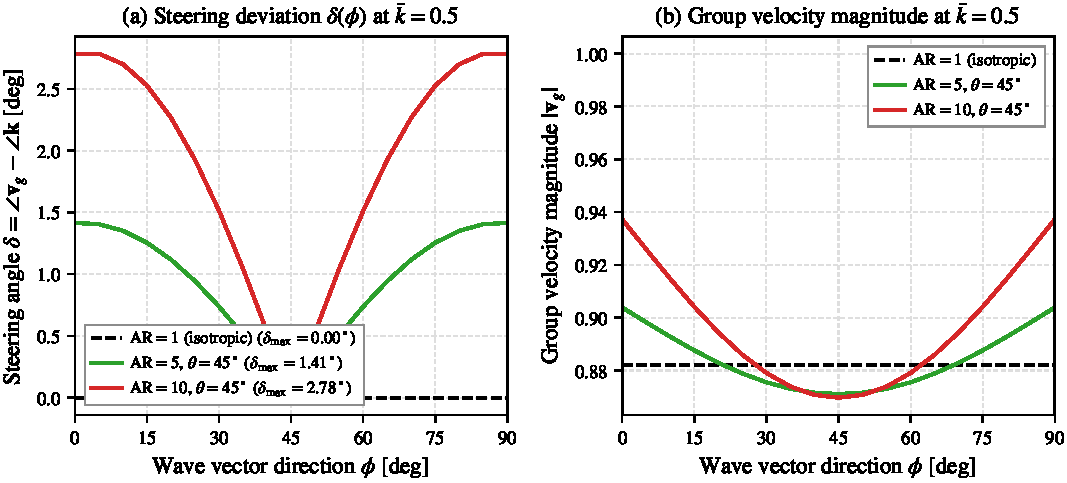
\includegraphics[width=\textwidth]{figures/fig12_ifc_wave_steering.pdf}
\caption{Acoustic-branch group-velocity steering on $|\bmk|=0.5$ at $\theta=45^\circ$. (a) Angular deviation for $\mathrm{AR}=1,5,10$, with peak values $0^\circ$, $1.4146^\circ$, and $2.7846^\circ$. (b) Directional variation of group-velocity magnitude.}
\label{fig:ifc_wave_steering}
\end{figure}

\subsection{Orientation repositions the steering lobes}
The orientation sweep in Figure~\ref{fig:s7_steering_sweep} and Table~\ref{tab:steering_sweep} evaluates $\theta\in\{0^\circ,15^\circ,\ldots,90^\circ\}$ for $\mathrm{AR}=5$ and $10$ on the same ring and acoustic branch. The peak deviation remains $1.4146^\circ$ and $2.7846^\circ$, respectively, across the sampled orientations to within $10^{-5}\,$deg. The principal direction follows $\phi^*(\theta)\simeq(45^\circ-\theta)\bmod90^\circ$, with excursions of at most $5^\circ$ at $\mathrm{AR}=10$. Thus, over the sampled grid, orientation shifts the steering lobes without materially changing their maximum amplitude.

\begin{figure}[htbp]
\centering
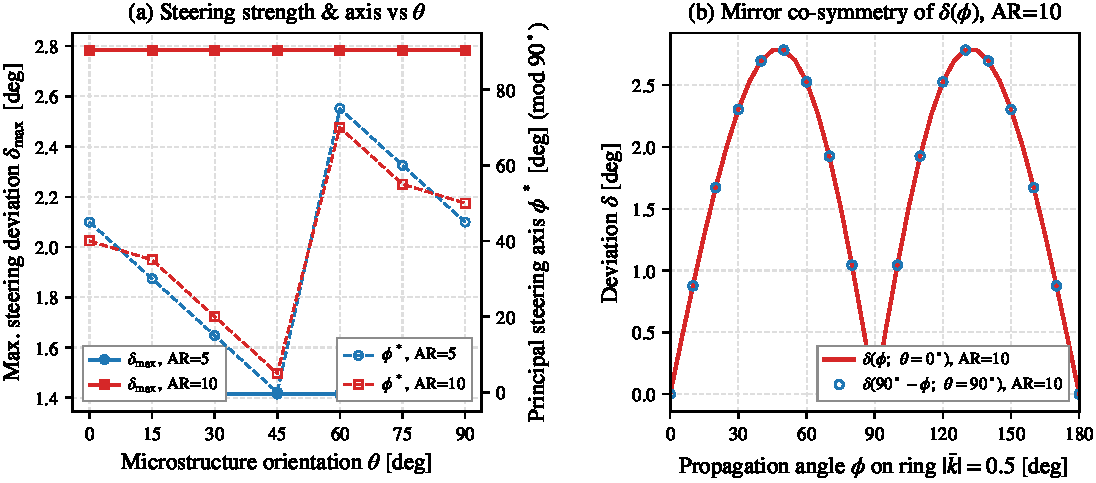
\includegraphics[width=\textwidth]{figures/fig14_s7_steering_sweep.pdf}
\caption{Orientation dependence of steering on $|\bmk|=0.5$. (a) Peak deviation $\delta_{\max}$ and principal direction $\phi^*$ for $\mathrm{AR}=5,10$; the peak amplitude is invariant over the sampled orientations, while the lobe direction follows the rotated tensor axes on the $5^\circ$ ring grid. (b) The $\theta=0^\circ$ and $90^\circ$ deviation fields at $\mathrm{AR}=10$ exhibit mirror co-symmetry.}
\label{fig:s7_steering_sweep}
\end{figure}

\begin{table}[htbp]
\centering
\caption{Peak group-velocity deviation and principal steering direction across the sampled orientations at $\bar{k}=0.5$.}
\label{tab:steering_sweep}
% Auto-generated by tab07_steering_sweep.py from p12b_s7_theta_sweep_mesh16.json - DO NOT EDIT MANUALLY
\begin{tabularx}{\textwidth}{@{}c r r r r@{}}
\toprule
$\theta$ & \multicolumn{2}{c}{$\mathrm{AR}=5$} & \multicolumn{2}{c}{$\mathrm{AR}=10$} \\
\cmidrule(lr){2-3}\cmidrule(lr){4-5}
 & $\delta_{\max}$ [deg] & $\phi^*$ [deg] & $\delta_{\max}$ [deg] & $\phi^*$ [deg] \\
\midrule
$0^\circ$ & 1.4146 & 45 & 2.7846 & 40 \\
$15^\circ$ & 1.4146 & 30 & 2.7846 & 35 \\
$30^\circ$ & 1.4146 & 15 & 2.7846 & 20 \\
$45^\circ$ & 1.4146 & 0 & 2.7846 & 5 \\
$60^\circ$ & 1.4146 & 75 & 2.7846 & 70 \\
$75^\circ$ & 1.4146 & 60 & 2.7846 & 55 \\
$90^\circ$ & 1.4146 & 45 & 2.7846 & 50 \\
\midrule
\multicolumn{5}{@{}>{\raggedright\arraybackslash}p{\dimexpr\textwidth-2\tabcolsep\relax}@{}}{$M_s = \phi^*(90^\circ) - \phi^*(0^\circ)$: $M_s(\mathrm{AR}{=}5) = +0.0000^\circ$, $M_s(\mathrm{AR}{=}10) = +10.0000^\circ$ (locked $5^\circ$ grid; parabolic refinement of the peak lies within one sampling step of these figures, so the sweep does not resolve any finer value)}\\
\multicolumn{5}{@{}>{\raggedright\arraybackslash}p{\dimexpr\textwidth-2\tabcolsep\relax}@{}}{Symmetries verified numerically ($\le 1.3\times 10^{-6}\,$deg for both headless and mirror): $\delta(\phi;\theta)=\delta(\phi+180^\circ;\theta)$ (headless) and $\delta(\phi;\theta)=\delta(90^\circ-\phi;\,90^\circ-\theta)$ (mirror).}\\
\bottomrule
\end{tabularx}

\end{table}

Defining the sampled steering measure as
\begin{equation}
M_s(\mathrm{AR})=\phi^*(90^\circ,\mathrm{AR})-\phi^*(0^\circ,\mathrm{AR}),
\label{eq:Ms_def}
\end{equation}
the values are
\begin{equation}
M_s(\mathrm{AR}=5)=0^\circ,\qquad M_s(\mathrm{AR}=10)=10^\circ.
\label{eq:Ms_value}
\end{equation}
The $5^\circ$ ring-sampling step limits the resolution of this difference. The deviation field also satisfies headless periodicity and mirror co-symmetry to residuals no greater than $1.3\times10^{-6}\,$deg; the peak amplitude is invariant under $\theta\mapsto90^\circ-\theta$ to within $10^{-7}\,$deg. These symmetries explain why orientation principally repositions the lobes rather than increasing the sampled peak deviation.

\subsection{Gradient energy and the high-wavenumber limit}
For Mindlin Form-II elasticity, the strain energy is the sum of the classical and gradient contributions, $W=W_c+W_g$, with $W_c=\tfrac12\int_\Omega\sigma_{ij}\varepsilon_{ij}\,\dif\Omega$ and $W_g=\tfrac12\int_\Omega\tau_{ijk}\eta_{ijk}\,\dif\Omega$. Along $\Gamma$--$X$, the gradient-energy fraction rises from $0.20\%$ at $\bar{k}=0.1$ to $16.49\%$ at $\bar{k}=1.0$ (Figure~\ref{fig:energy_microinertia}), showing the increasing contribution of double-stress work as the wavelength approaches the cell scale.

\begin{figure}[htbp]
\centering
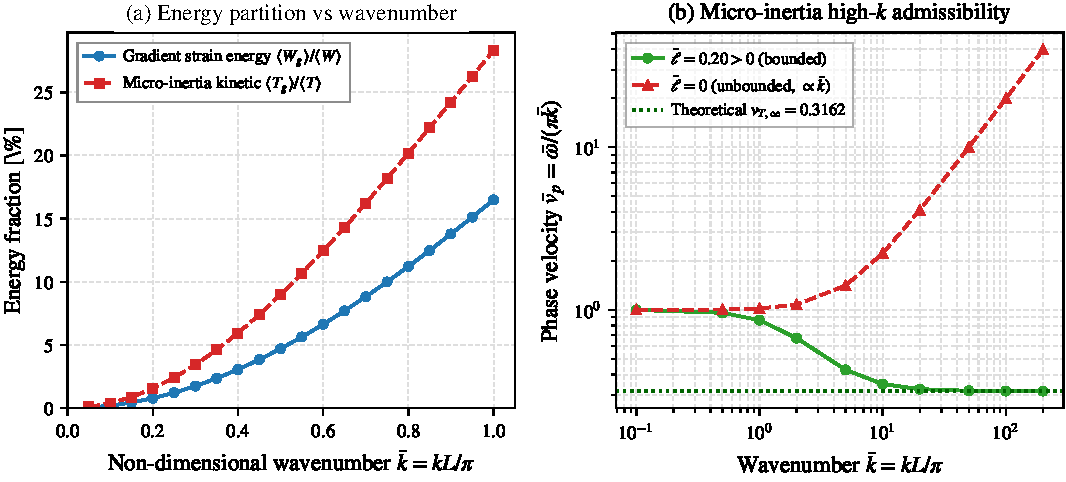
\includegraphics[width=\textwidth]{figures/fig13_energy_microinertia.pdf}
\caption{(a) Gradient-energy fraction $W_g/W$ versus wavenumber. (b) Transverse-branch phase velocity with and without gradient micro-inertia; the finite high-wavenumber limit is specific to the shear branch analyzed here.}
\label{fig:energy_microinertia}
\end{figure}

For the transverse shear branch considered in Appendix~\ref{app:asymptotics}, the model predicts
\begin{equation}
\bar{v}_{T,\infty}=\frac{\bar{l}_{\mathrm{eff}}}{\sqrt{10}\,\bar{\ell}_{\mathrm{i}}}=\frac{0.20}{\sqrt{10}\times0.20}=\frac{1}{\sqrt{10}}\approx0.3162.
\label{eq:v_horizon_sec7}
\end{equation}
At $\bar{k}=200$, the computed phase speed with micro-inertia is $0.3163$, within $0.03\%$ of this asymptote. In the corresponding no-micro-inertia model, the analytical branch relation grows without bound; the computed phase speed reaches $39.75$ at $\bar{k}=200$. This comparison concerns the stated transverse-branch model and does not establish a general speed bound for other branches or constitutive settings.

\section{Discussion and limitations}
\label{sec:discussion}

In homogeneous Case~H, rotating and elongating the characteristic-length tensor shifts the branches, changes directional gap widths, and redirects group velocity, while the complete-gap measure remains negative. Across the sampled steering grid, orientation moves the principal direction but leaves the peak deviation nearly unchanged. Orientation therefore controls directional dispersion and energy-flow direction in this case.

Case~C shows the effect of periodic impedance contrast, which produces a positive complete gap. The reported width falls from $2.5732$ on a $4\times4$ mesh to $1.9179$ on a $64\times64$ mesh and has not converged. The coarse-mesh value is resolution-specific; further refinement is needed before assigning a converged width. Case~H and Case~C use different material and discretization settings, so their gap values do not form a controlled parameter sweep.

The bilayer comparisons provide different levels of evidence. We check the classical AlN/BaTiO$_3$ calculation against the Rytov relation and compare it visually with the published plot. The two gradient-elastic cases are reproductions only; their source parameter conventions are unresolved, and numerical comparison data are unavailable (Supplementary Material~S2).

The analysis is linear, local, isothermal, and two-dimensional under plane-strain assumptions. It does not include nonlinear gradient effects, dissipation, piezoelectric coupling, or three-dimensional polarization modes. The finite high-wavenumber phase-speed result applies only to the transverse branch and constitutive model examined here.

\section{Conclusions}
\label{sec:conclusions}

\begin{enumerate}[label=\arabic*.,leftmargin=*,itemsep=0.45em]
  \item The conforming 32-degree-of-freedom BFS discretization applies the Bloch phase to displacement and derivative degrees of freedom. Seven of the eight tabulated consistency checks pass; the energy-flux/group-velocity identity remains marked for recheck after the harmonic micro-inertia sign correction. The classical bilayer transfer-matrix result reproduces the Rytov relation to $2.22\times10^{-16}$, while the published B1 comparison is visual and the B2/B3 source parameterization or numerical curves do not support quantitative comparison. These checks support internal consistency but do not establish quantitative external validation.
  \item The Case-H empirical mesh rate is $p=4.17$ (95\% CI $[3.15,5.20]$) over the $4^2$, $8^2$, and $16^2$ meshes; the $32^2$ result is resolution-limited and excluded from the fit. The rate describes the resolved meshes and is not a theoretical convergence-order claim.
  \item In Case~H, the isotropic reference has a $\Gamma$--$X$ width of $0.041$, and anisotropic configurations shift the branches to produce direction-specific stop bands. The largest sampled width is $\Delta_{GX}=0.0677$ at $\theta=0^\circ$, $\mathrm{AR}=7$; at $\theta=45^\circ$, $\mathrm{AR}=10$, it is $0.0043$. The complete-gap measure remains $\Delta_{\mathrm{complete}}\le-0.3235$. The implication is directional filtering, not full-zone attenuation.
  \item Across the 42 sampled configurations, the gap response is non-monotone, and the plotted surface interpolates sampled points rather than defining a continuous optimum. The orientation sensitivity reaches $S_\theta=2.34\,\mathrm{rad}^{-1}$ at $\mathrm{AR}=10$. The map is therefore useful for comparing sampled candidates, not for claiming a continuous optimum.
  \item On the acoustic branch at $\bar{k}=0.5$, the peak steering deviation rises from $0^\circ$ at $\mathrm{AR}=1$ to $1.4146^\circ$ at $\mathrm{AR}=5$ and $2.7846^\circ$ at $\mathrm{AR}=10$. Over the sampled orientations, the peak remains invariant within $10^{-5}\,$deg while the steering lobes move; the sampled measure $M_s$ is $0^\circ$ and $10^\circ$ for $\mathrm{AR}=5$ and $10$, respectively, on the $5^\circ$ ring grid. Thus orientation redirects the energy-flow direction without materially changing the sampled peak deviation.
  \item In the separate heterogeneous Case~C calculation, periodic epoxy--YBCO contrast produces a positive complete gap of $2.5732$ ($43.94\%$) on the $4\times4$ mesh. The width falls to $1.9179$ at $64\times64$ and has not converged. Unlike the directional Case-H gaps, this coarse-mesh Case-C result spans the sampled Brillouin zone; its width remains mesh-sensitive and the two cases do not constitute a controlled sweep.
  \item Along $\Gamma$--$X$, the gradient-energy fraction rises from $0.20\%$ at $\bar{k}=0.1$ to $16.49\%$ at $\bar{k}=1.0$. For the transverse branch studied, gradient micro-inertia gives the high-wavenumber phase-speed limit $\bar{v}_{T,\infty}=0.3162$; at $\bar{k}=200$ the computed value is $0.3163$, whereas the no-micro-inertia branch reaches $39.75$. The bound is specific to this branch and constitutive model, not a general bound for all modes.
\end{enumerate}


\appendix
\section{High-Wavenumber Phase Velocity Asymptotics}
\label{app:asymptotics}

We derive the high-wavenumber phase-speed limit for the one-dimensional transverse-shear branch of the strain-gradient model. Without micro-inertia ($\ell_{\mathrm{i}}=0$), the phase velocity grows without bound as $k\to\infty$. With micro-inertia ($\ell_{\mathrm{i}}>0$), it approaches a finite asymptote.

We consider one-dimensional transverse-shear propagation in a Mindlin Form-II gradient-elastic continuum governed by the equation of motion:
\begin{equation}
\mu \frac{\partial^2 u}{\partial x^2} - \frac{1}{10} \mu l_{\mathrm{eff}}^2 \frac{\partial^4 u}{\partial x^4} = \rho \frac{\partial^2 u}{\partial t^2} - \rho \ell_{\mathrm{i}}^2 \frac{\partial^4 u}{\partial x^2 \partial t^2},
\label{eq:appA_pde}
\end{equation}
where $\mu$ is the shear modulus, $\rho$ is the mass density, $l_{\mathrm{eff}}^2 = \hat{\bmk}\cdot\mathbf{L}\cdot\hat{\bmk}$ is the effective characteristic gradient-stiffness length scale (with the factor $1/10$ inherited from the second moment of the 3D ellipsoidal domain), and $\ell_{\mathrm{i}}$ is the micro-inertia length parameter. Substituting the time-harmonic plane wave ansatz $u(x, t) = A e^{\iu(k x - \omega t)}$ into Eq.~\eqref{eq:appA_pde} yields:
\begin{equation}
-\mu k^2 - \frac{1}{10} \mu l_{\mathrm{eff}}^2 k^4 = -\rho \omega^2 - \rho \ell_{\mathrm{i}}^2 \omega^2 k^2.
\label{eq:appA_char}
\end{equation}
Solving the equation gives the dispersion relation:
\begin{equation}
\omega^2(k) = \frac{\mu}{\rho} \frac{k^2 \left( 1 + \frac{1}{10} l_{\mathrm{eff}}^2 k^2 \right)}{1 + \ell_{\mathrm{i}}^2 k^2}.
\label{eq:appA_dispersion}
\end{equation}
The phase velocity $v_p(k) \equiv \omega(k)/k$ is therefore:
\begin{equation}
v_p(k) = \sqrt{\frac{\mu}{\rho}} \sqrt{\frac{1 + \frac{1}{10} l_{\mathrm{eff}}^2 k^2}{1 + \ell_{\mathrm{i}}^2 k^2}} = c_T \sqrt{\frac{1 + \frac{1}{10} l_{\mathrm{eff}}^2 k^2}{1 + \ell_{\mathrm{i}}^2 k^2}},
\label{eq:appA_vp}
\end{equation}
where $c_T = \sqrt{\mu/\rho}$ is the classical acoustic shear wave speed.

\paragraph{Case 1: No micro-inertia ($\ell_{\mathrm{i}} = 0$)}
Setting $\ell_{\mathrm{i}} = 0$ in Eq.~\eqref{eq:appA_vp} yields:
\begin{equation}
v_p(k) = c_T \sqrt{1 + \frac{1}{10} l_{\mathrm{eff}}^2 k^2}.
\label{eq:appA_vp_zero}
\end{equation}
In the short-wave limit ($k \to \infty$), the phase velocity behaves asymptotically as:
\begin{equation}
\lim_{k \to \infty} v_p(k) = \lim_{k \to \infty} \frac{c_T l_{\mathrm{eff}}}{\sqrt{10}} k \to \infty.
\label{eq:appA_unbounded}
\end{equation}
Similarly, the group velocity $v_g(k) = \dif\omega/\dif k$ is given by:
\begin{equation}
v_g(k) = c_T \frac{1 + \frac{2}{10} l_{\mathrm{eff}}^2 k^2}{\sqrt{1 + \frac{1}{10} l_{\mathrm{eff}}^2 k^2}} \sim \frac{2 c_T l_{\mathrm{eff}}}{\sqrt{10}} k \to \infty \quad \text{as } k \to \infty.
\label{eq:appA_vg_unbounded}
\end{equation}
Both phase and group velocities therefore grow without bound at high wavenumbers in this one-dimensional transverse-shear model when micro-inertia is omitted.

\paragraph{Case 2: With micro-inertia ($\ell_{\mathrm{i}} > 0$)}
For $\ell_{\mathrm{i}} > 0$, taking the limit of Eq.~\eqref{eq:appA_vp} as $k \to \infty$ gives:
\begin{equation}
v_{p,\infty} \equiv \lim_{k \to \infty} v_p(k) = c_T \lim_{k \to \infty} \sqrt{\frac{\frac{1}{10} l_{\mathrm{eff}}^2 k^2 (1 + \frac{10}{l_{\mathrm{eff}}^2 k^2})}{\ell_{\mathrm{i}}^2 k^2 (1 + \frac{1}{\ell_{\mathrm{i}}^2 k^2})}} = c_T \frac{l_{\mathrm{eff}}}{\sqrt{10}\,\ell_{\mathrm{i}}}.
\label{eq:appA_vp_bounded}
\end{equation}
With velocity scaled by $c_T = 1.0$, the dimensionless limit is:
\begin{equation}
\bar{v}_{T,\infty} = \frac{\bar{l}_{\mathrm{eff}}}{\sqrt{10}\,\bar{\ell}_{\mathrm{i}}}.
\label{eq:appA_v_horizon}
\end{equation}
For the Case H baseline ($l_{\mathrm{eff}} = l_{\mathrm{iso}} = 0.20\,\mathrm{m}$, $\ell_{\mathrm{i}} = 0.20\,\mathrm{m}$ from Table~\ref{tab:case_params}, with $\bar{l}_{\mathrm{eff}} = 0.20$ and $\bar{\ell}_{\mathrm{i}} = 0.20$), the transverse asymptotic limit is:
\begin{equation}
\bar{v}_{T,\infty} = \frac{0.20}{\sqrt{10} \times 0.20} = \frac{1}{\sqrt{10}} \approx 0.3162.
\label{eq:appA_horizon_val}
\end{equation}
As verified numerically in Section~\ref{sec:microinertia}, the finite element phase velocity at $\bar{k} = 200$ attains $\bar{v}_p = 0.3163$, matching the analytical horizon within $0.03\%$. For this transverse branch, micro-inertia gives a finite high-wavenumber phase-speed limit.

\section{Time-Averaged Energy Flux in Form-II Gradient Elasticity}
\label{app:energy_flux}

In this appendix, we derive the conservation of elastodynamic energy and the explicit form of the time-averaged Poynting-type energy flux vector $\bm{S}$ in a Mindlin Form-II gradient-elastic solid with micro-inertia.

The local balance of mechanical energy is expressed by the continuity relation:
\begin{equation}
\frac{\partial}{\partial t}(W + T) + \nabla \cdot \bm{S} = 0,
\label{eq:appB_poynting_theorem}
\end{equation}
where $W$ and $T$ are the strain and kinetic energy densities defined in Eqs.~\eqref{eq:strain_energy_W} and \eqref{eq:kinetic_energy_T}. Differentiating $W$ and $T$ with respect to time gives:
\begin{align}
\frac{\partial W}{\partial t} &= \sigma_{ij} \dot{\varepsilon}_{ij} + \tau_{ijk} \dot{\eta}_{ijk} = \sigma_{ij} \dot{u}_{i,j} + \tau_{ijk} \dot{u}_{i,jk}, \label{eq:appB_dWdt} \\
\frac{\partial T}{\partial t} &= \rho \dot{u}_i \ddot{u}_i + \rho \ell_{\mathrm{i}}^2 \dot{u}_{i,j} \ddot{u}_{i,j}. \label{eq:appB_dTdt}
\end{align}
Expanding the spatial derivative terms in Eq.~\eqref{eq:appB_dWdt} using the product rule:
\begin{align}
\sigma_{ij} \dot{u}_{i,j} &= (\sigma_{ij} \dot{u}_i)_{,j} - \sigma_{ij,j} \dot{u}_i, \label{eq:appB_id1} \\
\tau_{ijk} \dot{u}_{i,jk} &= (\tau_{ijk} \dot{u}_{i,j})_{,k} - \tau_{ijk,k} \dot{u}_{i,j} = (\tau_{ikj} \dot{u}_{i,k})_{,j} - (\tau_{ijk,k} \dot{u}_i)_{,j} + \tau_{ijk,kj} \dot{u}_i. \label{eq:appB_id2}
\end{align}
Similarly, the micro-inertial rate term in Eq.~\eqref{eq:appB_dTdt} expands to:
\begin{equation}
\rho \ell_{\mathrm{i}}^2 \dot{u}_{i,j} \ddot{u}_{i,j} = (\rho \ell_{\mathrm{i}}^2 \dot{u}_i \ddot{u}_{i,j})_{,j} - \rho \ell_{\mathrm{i}}^2 \dot{u}_i \ddot{u}_{i,jj}.
\label{eq:appB_id3}
\end{equation}
Adding Eqs.~\eqref{eq:appB_dWdt} and \eqref{eq:appB_dTdt} and substituting the equation of motion $\sigma_{ij,j} - \tau_{ijk,jk} = \rho(\ddot{u}_i - \ell_{\mathrm{i}}^2 \ddot{u}_{i,jj})$ from Eq.~\eqref{eq:strong_form} cancels the bulk terms:
\begin{equation}
\frac{\partial (W + T)}{\partial t} = \left[ (\sigma_{ij} - \tau_{ijk,k}) \dot{u}_i + \tau_{ikj} \dot{u}_{i,k} + \rho \ell_{\mathrm{i}}^2 \dot{u}_i \ddot{u}_{i,j} \right]_{,j}.
\label{eq:appB_energy_step}
\end{equation}
Comparing Eq.~\eqref{eq:appB_energy_step} with Eq.~\eqref{eq:appB_poynting_theorem} gives the instantaneous energy flux vector $S_j$:
\begin{equation}
S_j = -(\sigma_{ij} - \tau_{ijk,k}) \dot{u}_i - \tau_{ikj} \dot{u}_{i,k} - \rho \ell_{\mathrm{i}}^2 \dot{u}_i \ddot{u}_{i,j}.
\label{eq:appB_S_instant}
\end{equation}
The terms in Eq.~\eqref{eq:appB_S_instant} describe classical traction power modified by the double-stress divergence, double-stress power acting on velocity gradients, and a micro-inertial term.

For time-harmonic fields represented in complex notation $\bmu(\bmx, t) = \mathrm{Re}[\tilde{\bmu}(\bmx) e^{-\iu \omega t}]$, the cycle-averaged energy flux $\langle S_j \rangle = \frac{1}{\mathcal{T}}\int_0^{\mathcal{T}} S_j\,\dif t$ is given by:
\begin{equation}
\langle S_j \rangle = -\frac{1}{2} \mathrm{Re} \left[ (\tilde{\sigma}_{ij} - \tilde{\tau}_{ijk,k}) (-\iu \omega \tilde{u}_i)^* + \tilde{\tau}_{ikj} (-\iu \omega \tilde{u}_{i,k})^* + \rho \ell_{\mathrm{i}}^2 (-\iu \omega \tilde{u}_i) (-\omega^2 \tilde{u}_{i,j})^* \right].
\label{eq:appB_S_cycle}
\end{equation}
Integrating over the unit cell $\Omega_{\mathrm{cell}}$, the cycle-averaged energy flux $\langle \bm{S} \rangle$ and stored energy satisfy:
\begin{equation}
\bm{v}_g = \frac{\langle \bm{S} \rangle}{\langle W \rangle + \langle T \rangle},
\label{eq:appB_vg_identity}
\end{equation}
This identity relates the group velocity $\bm{v}_g = \nabla_{\bmk}\omega$ to the cell-averaged energy flux and stored energy. The earlier consistency table lists a group-velocity/energy-flux residual of $6.91\times10^{-10}$ (Table~\ref{tab:consistency_suite}). Because the harmonic micro-inertial sign in Eq.~\eqref{eq:appB_S_cycle} has been corrected, this residual remains a prior result pending rerun, not a current verification.


\section*{Data availability statement}
The data supporting the findings of this study are available within the
article.

\section*{Conflict of interest disclosure statement}
No potential conflict of interest was reported by the authors.

\section*{Acknowledgments}
The authors gratefully acknowledge the financial support provided by the
Haryana State Higher Education Council (HSHEC), Government of Haryana,
under the Haryana State Research Fund (HSRF) scheme (Sanction Order
No.~14/66-2025 SPD/HSHEC/HSRF).

\newpage
\bibliographystyle{elsarticle-num}
\bibliography{references}

\end{document}
